%---------------------------------%
% Article Body
%---------------------------------%
\documentclass[../article.tex, 12pt]{subfiles}
\begin{document}

%---------------------------------%
% Title
%---------------------------------%
%\begin{center}
%{\bfseries\Huge Cultivator Report: Flow Gardens}
%\end{center}
%
%%\vspace*{-1\baselineskip}
%\begin{center}
%{\Large By Keegan Skeate}
%\end{center}
%\vspace*{1\baselineskip}

%---------------------------------%
% Abstract
%---------------------------------%
%\pdfbookmark[1]{Abstract}{Abstract}
%\Abstract{\hspace{4ex}
%Begin...
%}

%---------------------------------%
% Data
%---------------------------------%
%\begin{multicols}{2}
\section*{Data}
\label{sec:Data}
%\thispagestyle{titlepage}
\pagestyle{regular}

This is a report on California lab results, extracted from certificates of analysis (COAs) published by the Flower Company on their cannabis distribution website\footnote[1]{Note: Data collected from \href{https://flowercompany.com}{https://flowercompany.com}.}, collected between December \nth{15}, 2023 and February \nth{20} 2024. We hope these statistics can help shed light on cannabis in California.

\vspace{1\baselineskip}

\noindent California Lab Result Data\\[0.25\baselineskip]
    \subfile{stats/summary}
    
\vspace{2\baselineskip}

% Pie charts
\noindent%
\begin{minipage}[t]{0.45\textwidth}

    % Proportion of categories.
    \centering
    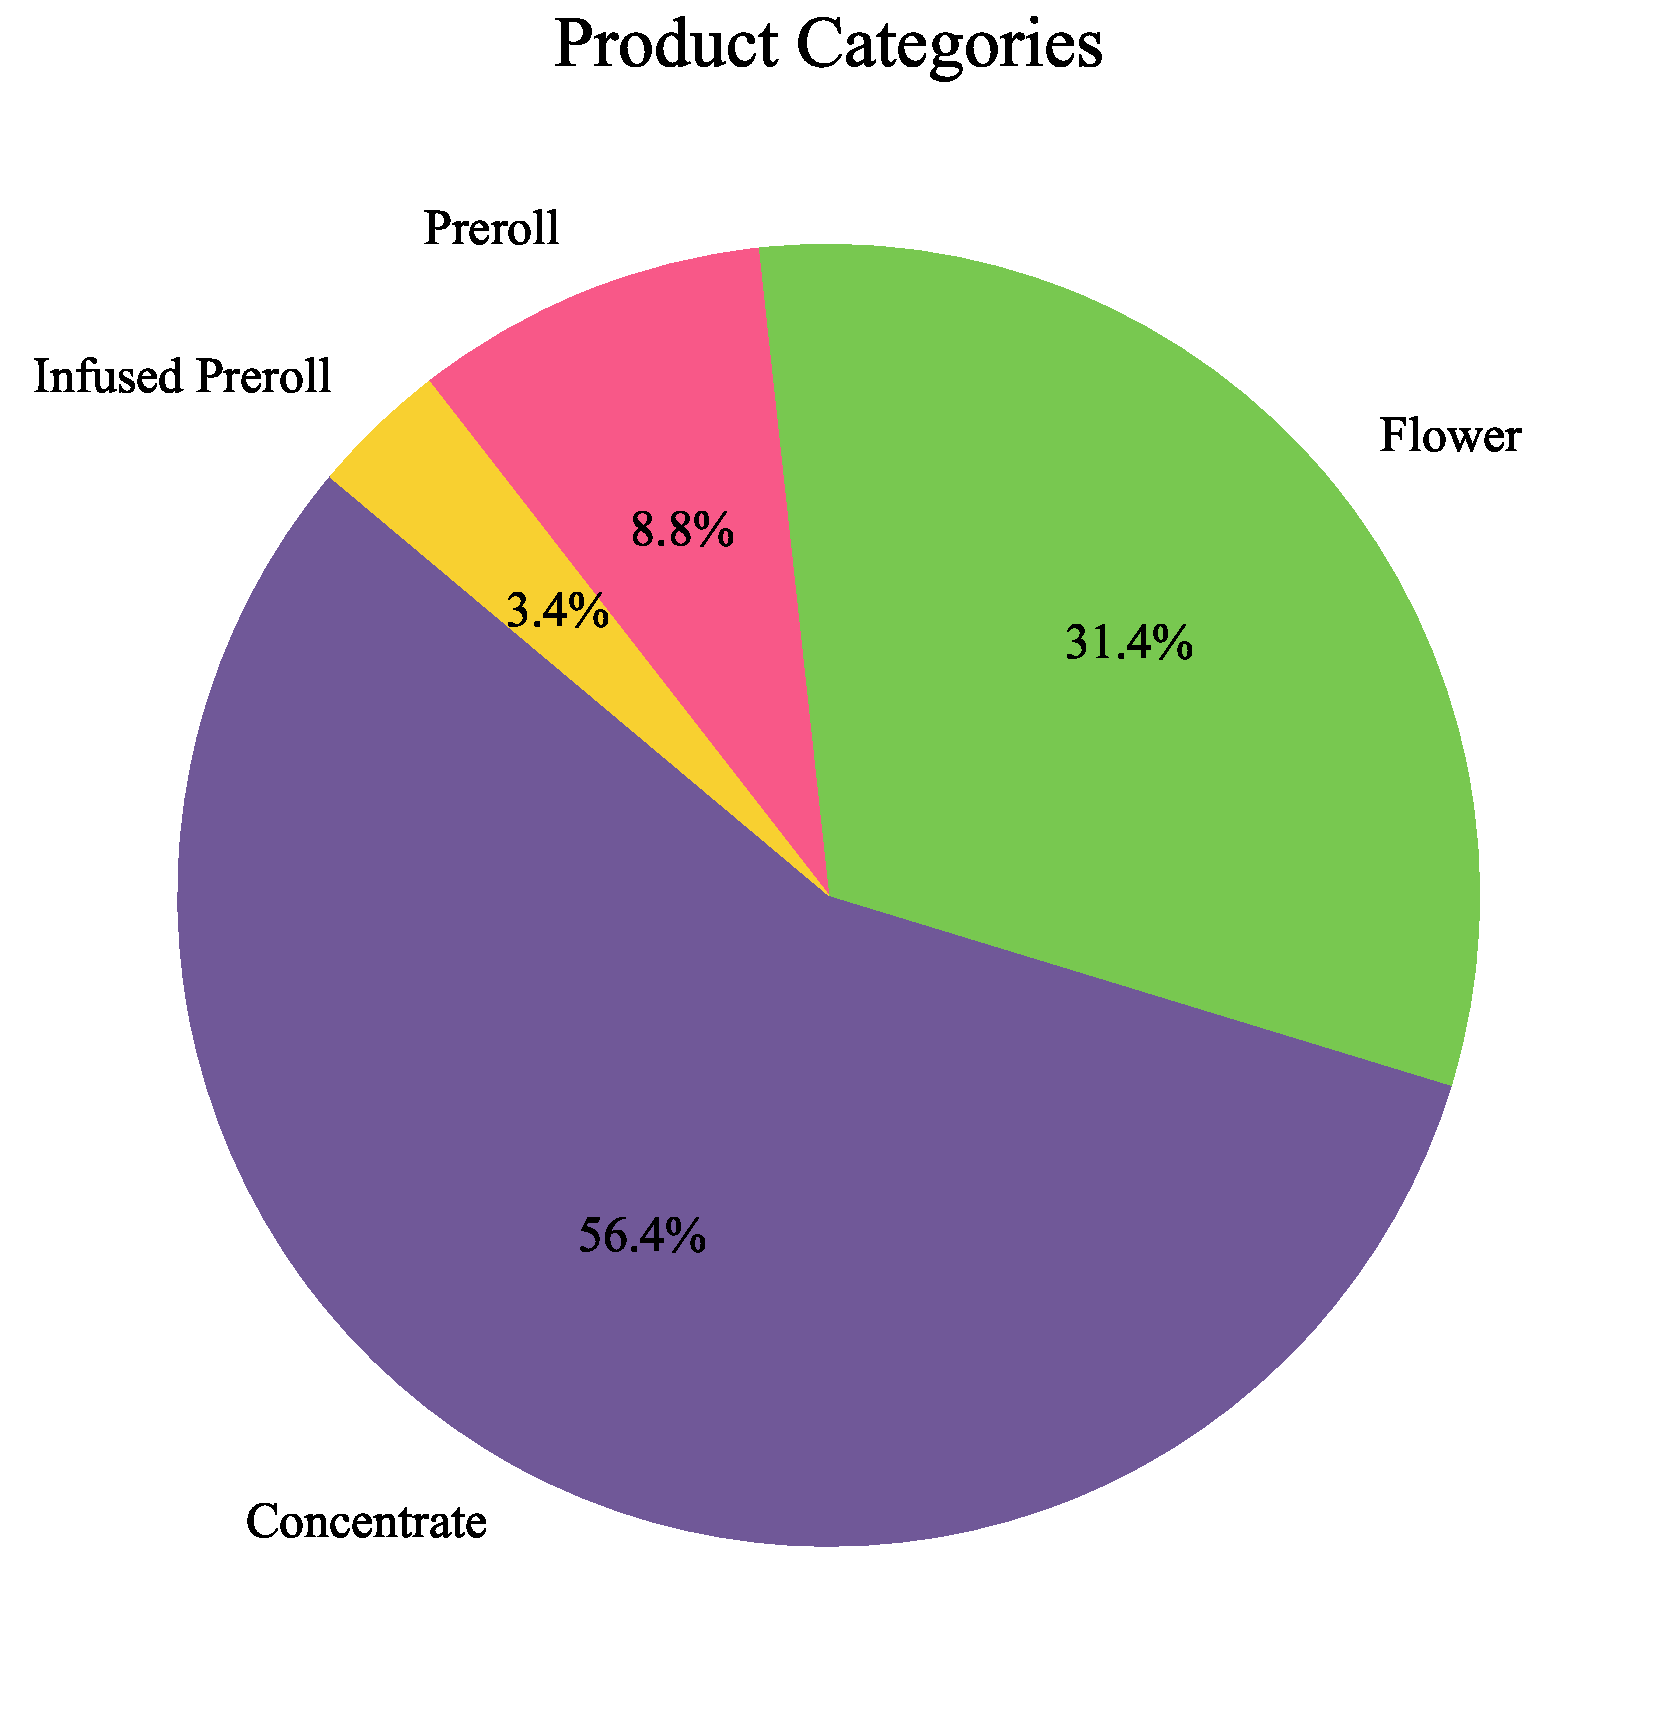
\includegraphics[width=0.9\linewidth]{figures/product-categories-pie-chart.pdf}

\end{minipage}\hspace{0.05\textwidth}
%
\begin{minipage}[t]{0.45\textwidth}

    % Proportion of concentrate subtypes.
    \centering
    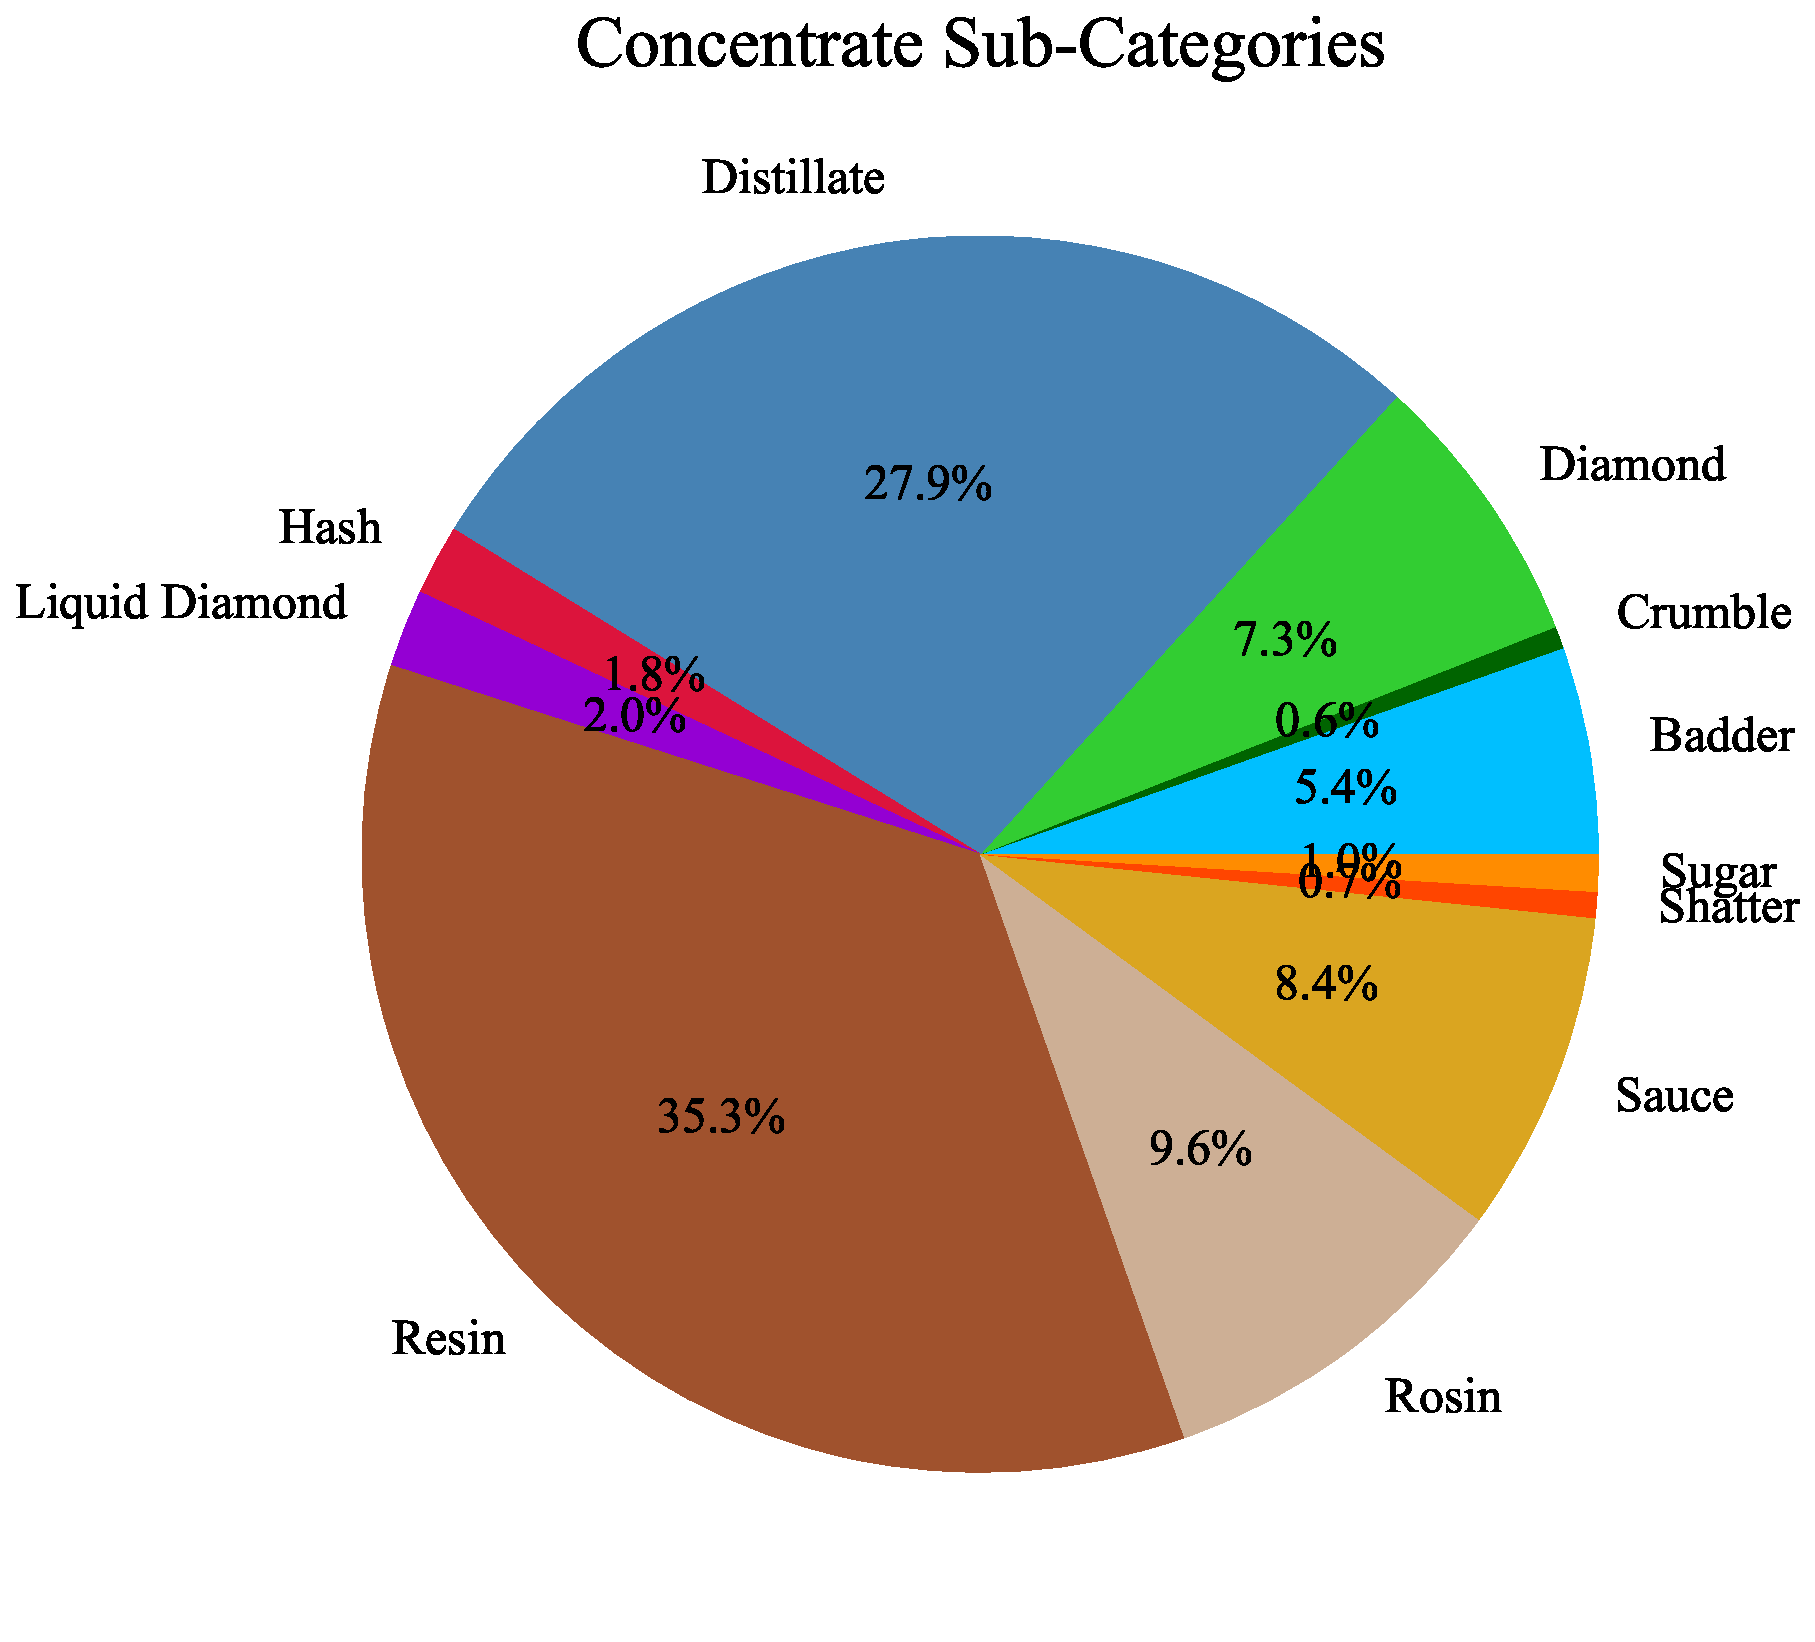
\includegraphics[width=\linewidth]{figures/concentrate-subcategories-pie-chart.pdf}

\end{minipage}

\vspace{1\baselineskip}

\noindent%
\begin{minipage}[t]{0.45\textwidth}

    % Value counts of producers.
    \subfile{stats/top-producers}

\end{minipage}\hspace{0.05\textwidth}
%
\begin{minipage}[t]{0.45\textwidth}

    % Value counts of labs.
    \subfile{stats/top-labs}

\end{minipage}


%---------------------------------%
% Chemical Analysis
%---------------------------------%
\newpage
\section*{Chemical Analysis}
\label{sec:Chemical Analysis}

First, we examine total cannabinoids and total terpenes in flower and concentrates.

\vspace{2\baselineskip}

% Total cannabinoids to total terpenes in flower
\begin{center}
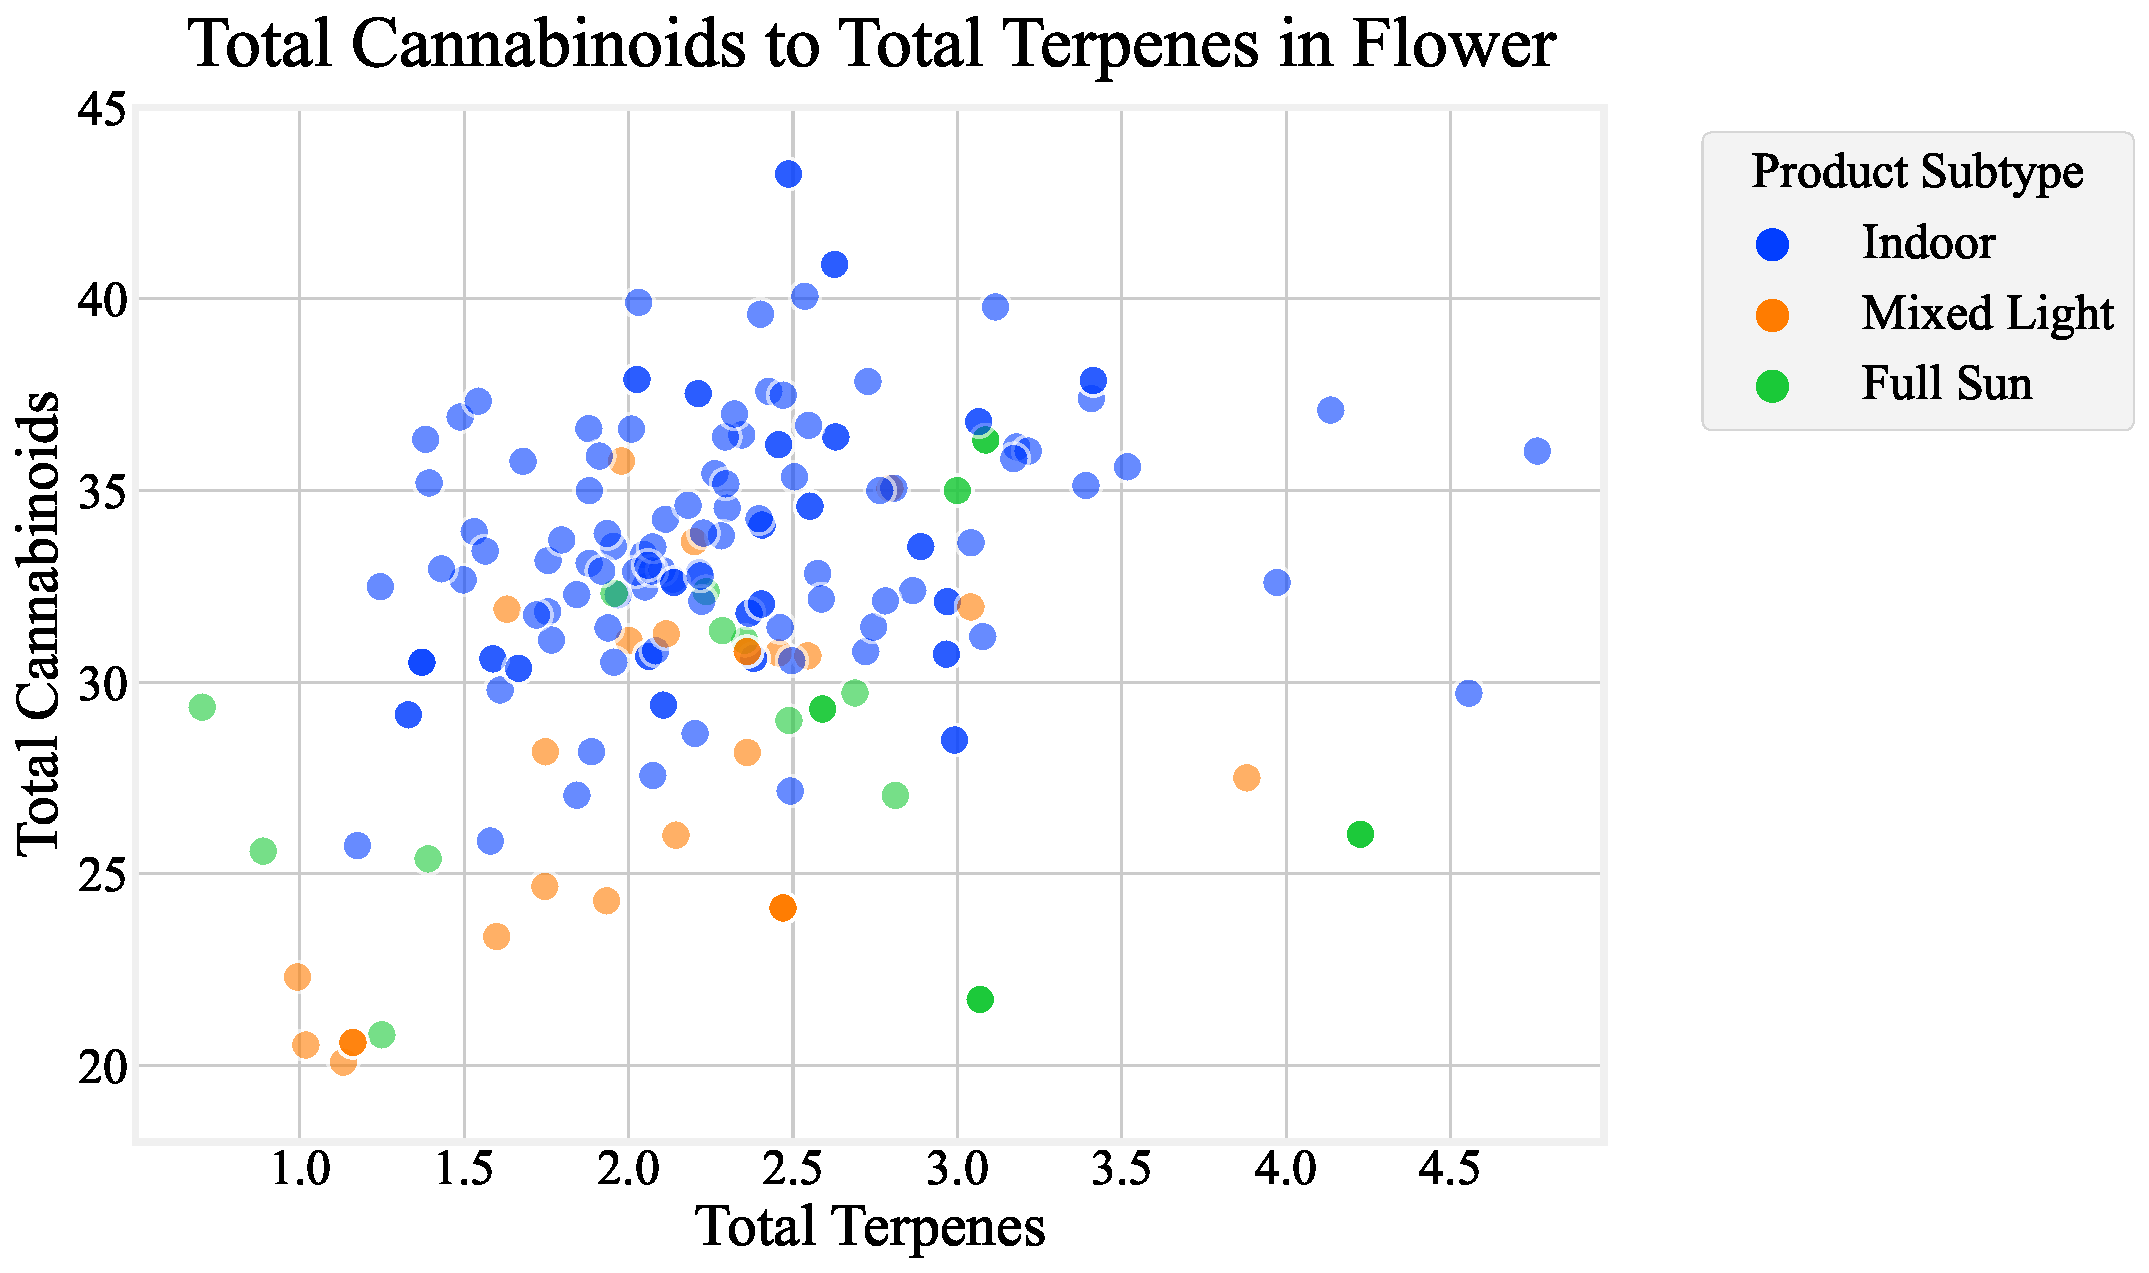
\includegraphics[width=0.8\linewidth]{figures/total-cannabinoids-total-terpenes-flower.pdf}
\end{center}

\vspace{2\baselineskip}

% Total cannabinoids to total terpenes in concentrates
\begin{center}
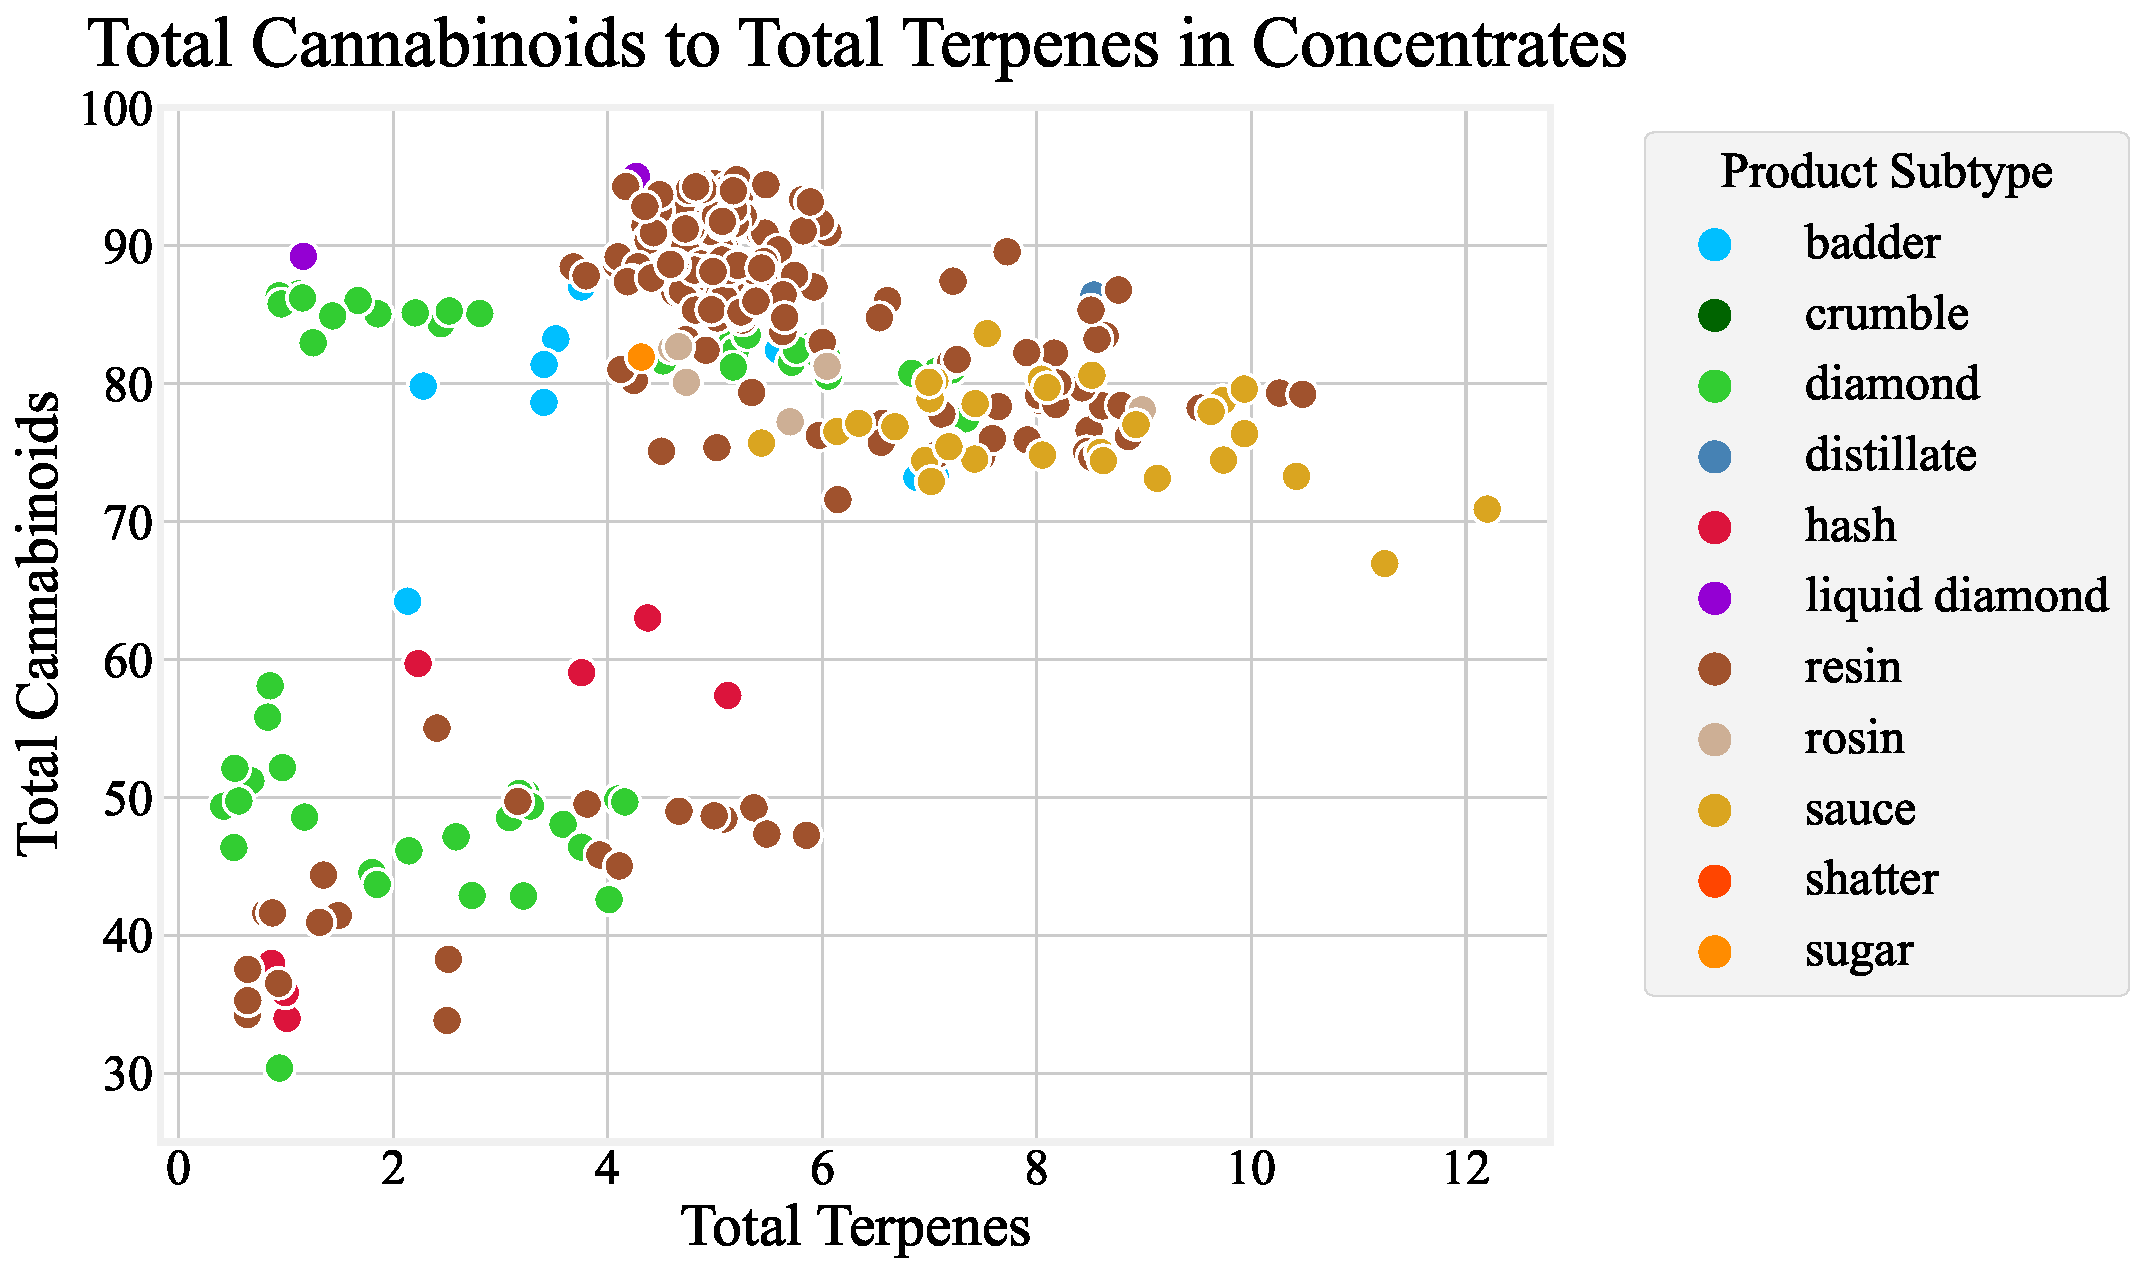
\includegraphics[width=0.8\linewidth]{figures/total-cannabinoids-total-terpenes-concentrates.pdf}
\end{center}

\newpage
Next, we visualize THCA and $\Delta$-9 THC concentrations.

\vspace{2\baselineskip}

% THCA to delta-9 THC in flower
\begin{center}
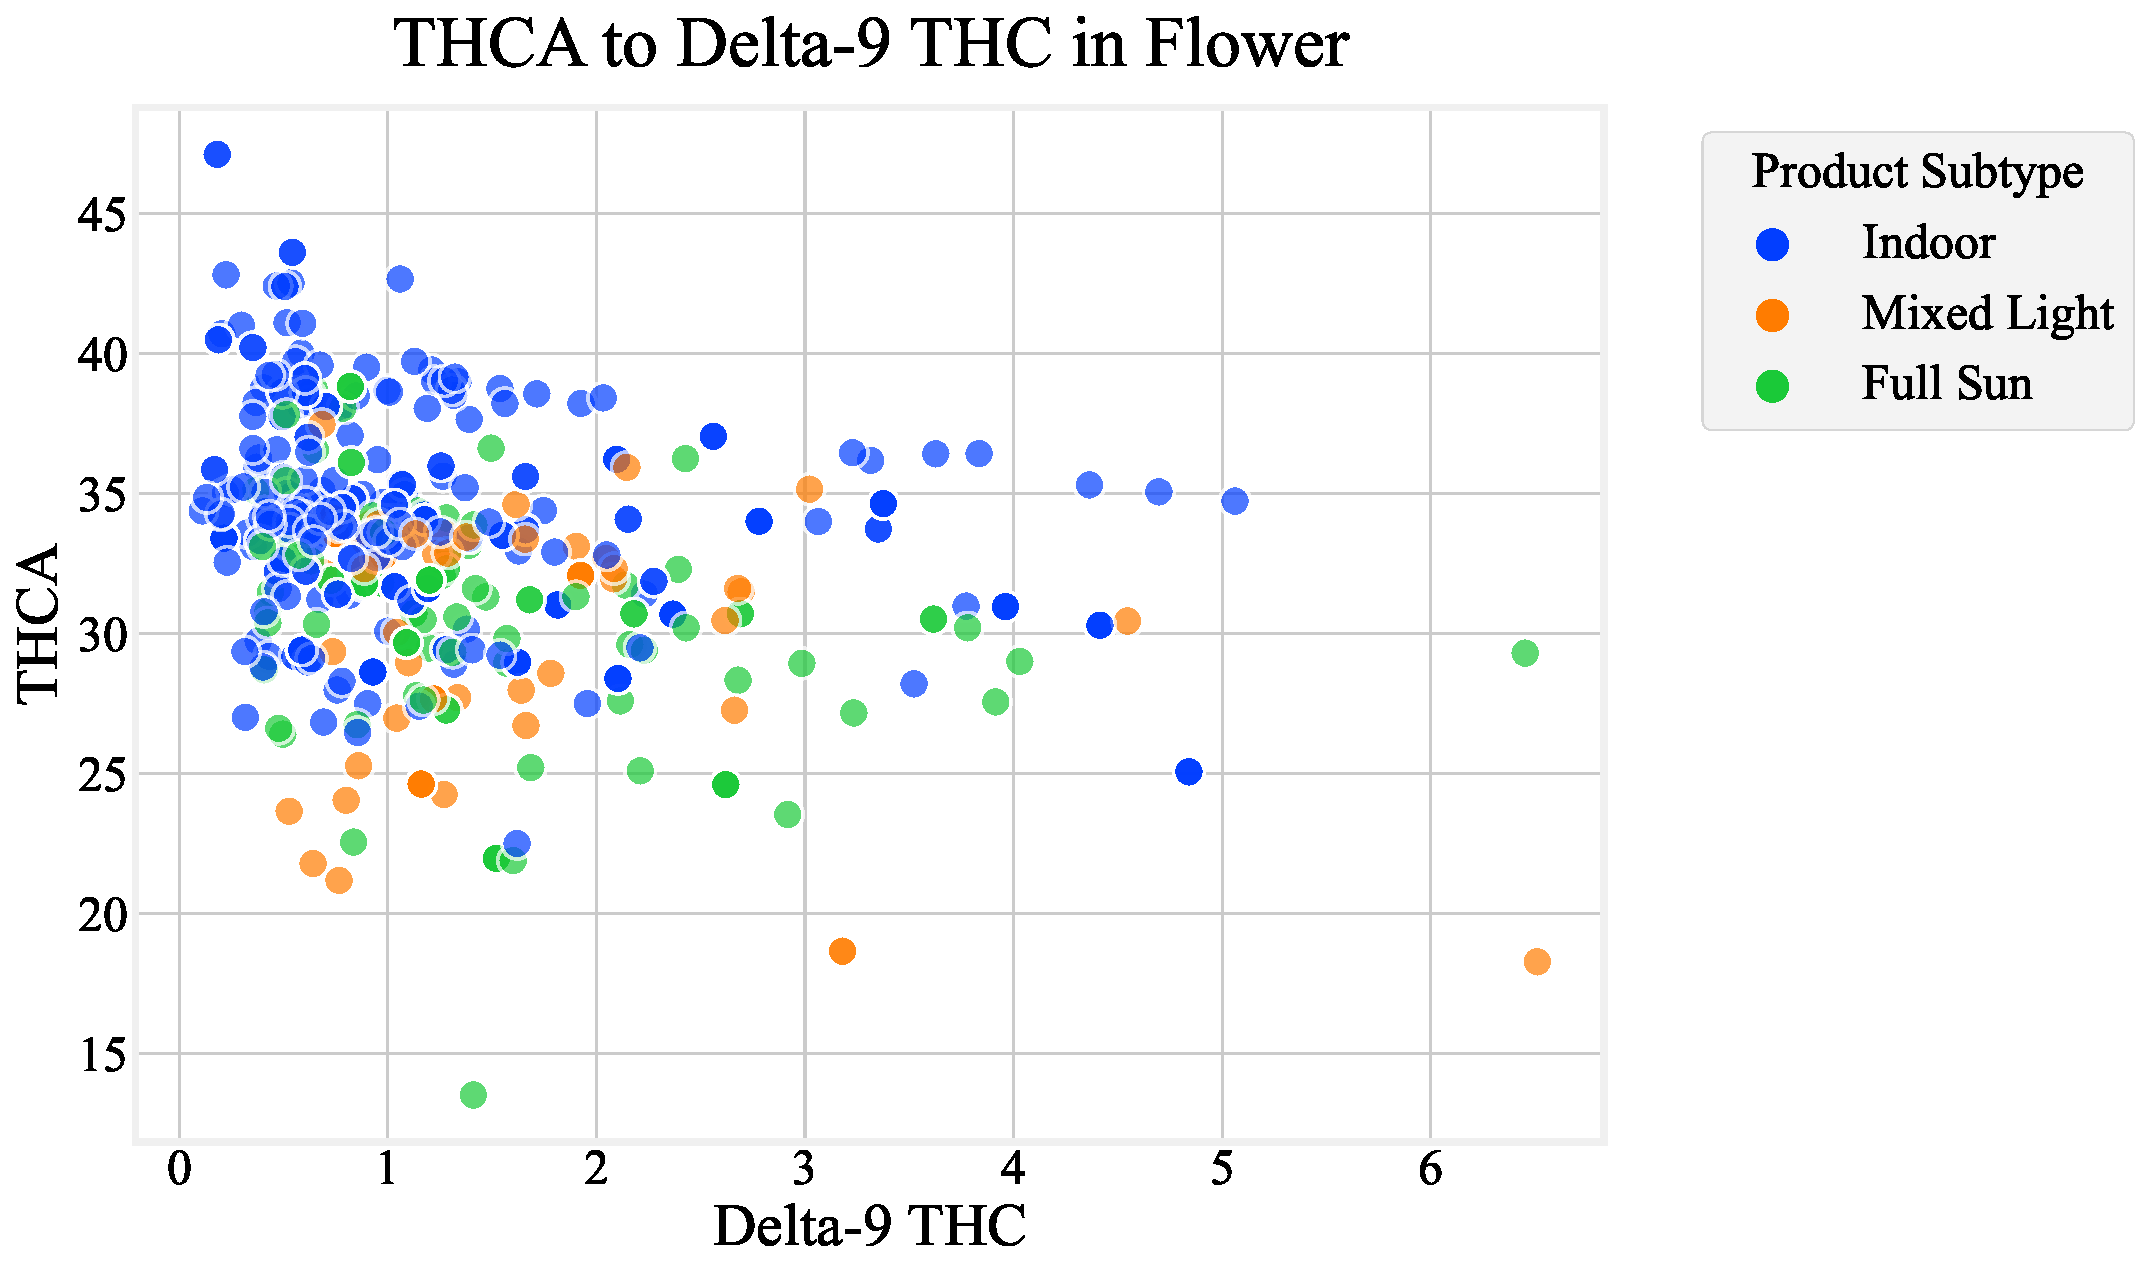
\includegraphics[width=0.8\linewidth]{figures/thca-to-delta-9-thc-flower.pdf}

\end{center}
\vspace{2\baselineskip}

% THCA to delta-9 THC in concentrates
\begin{center}
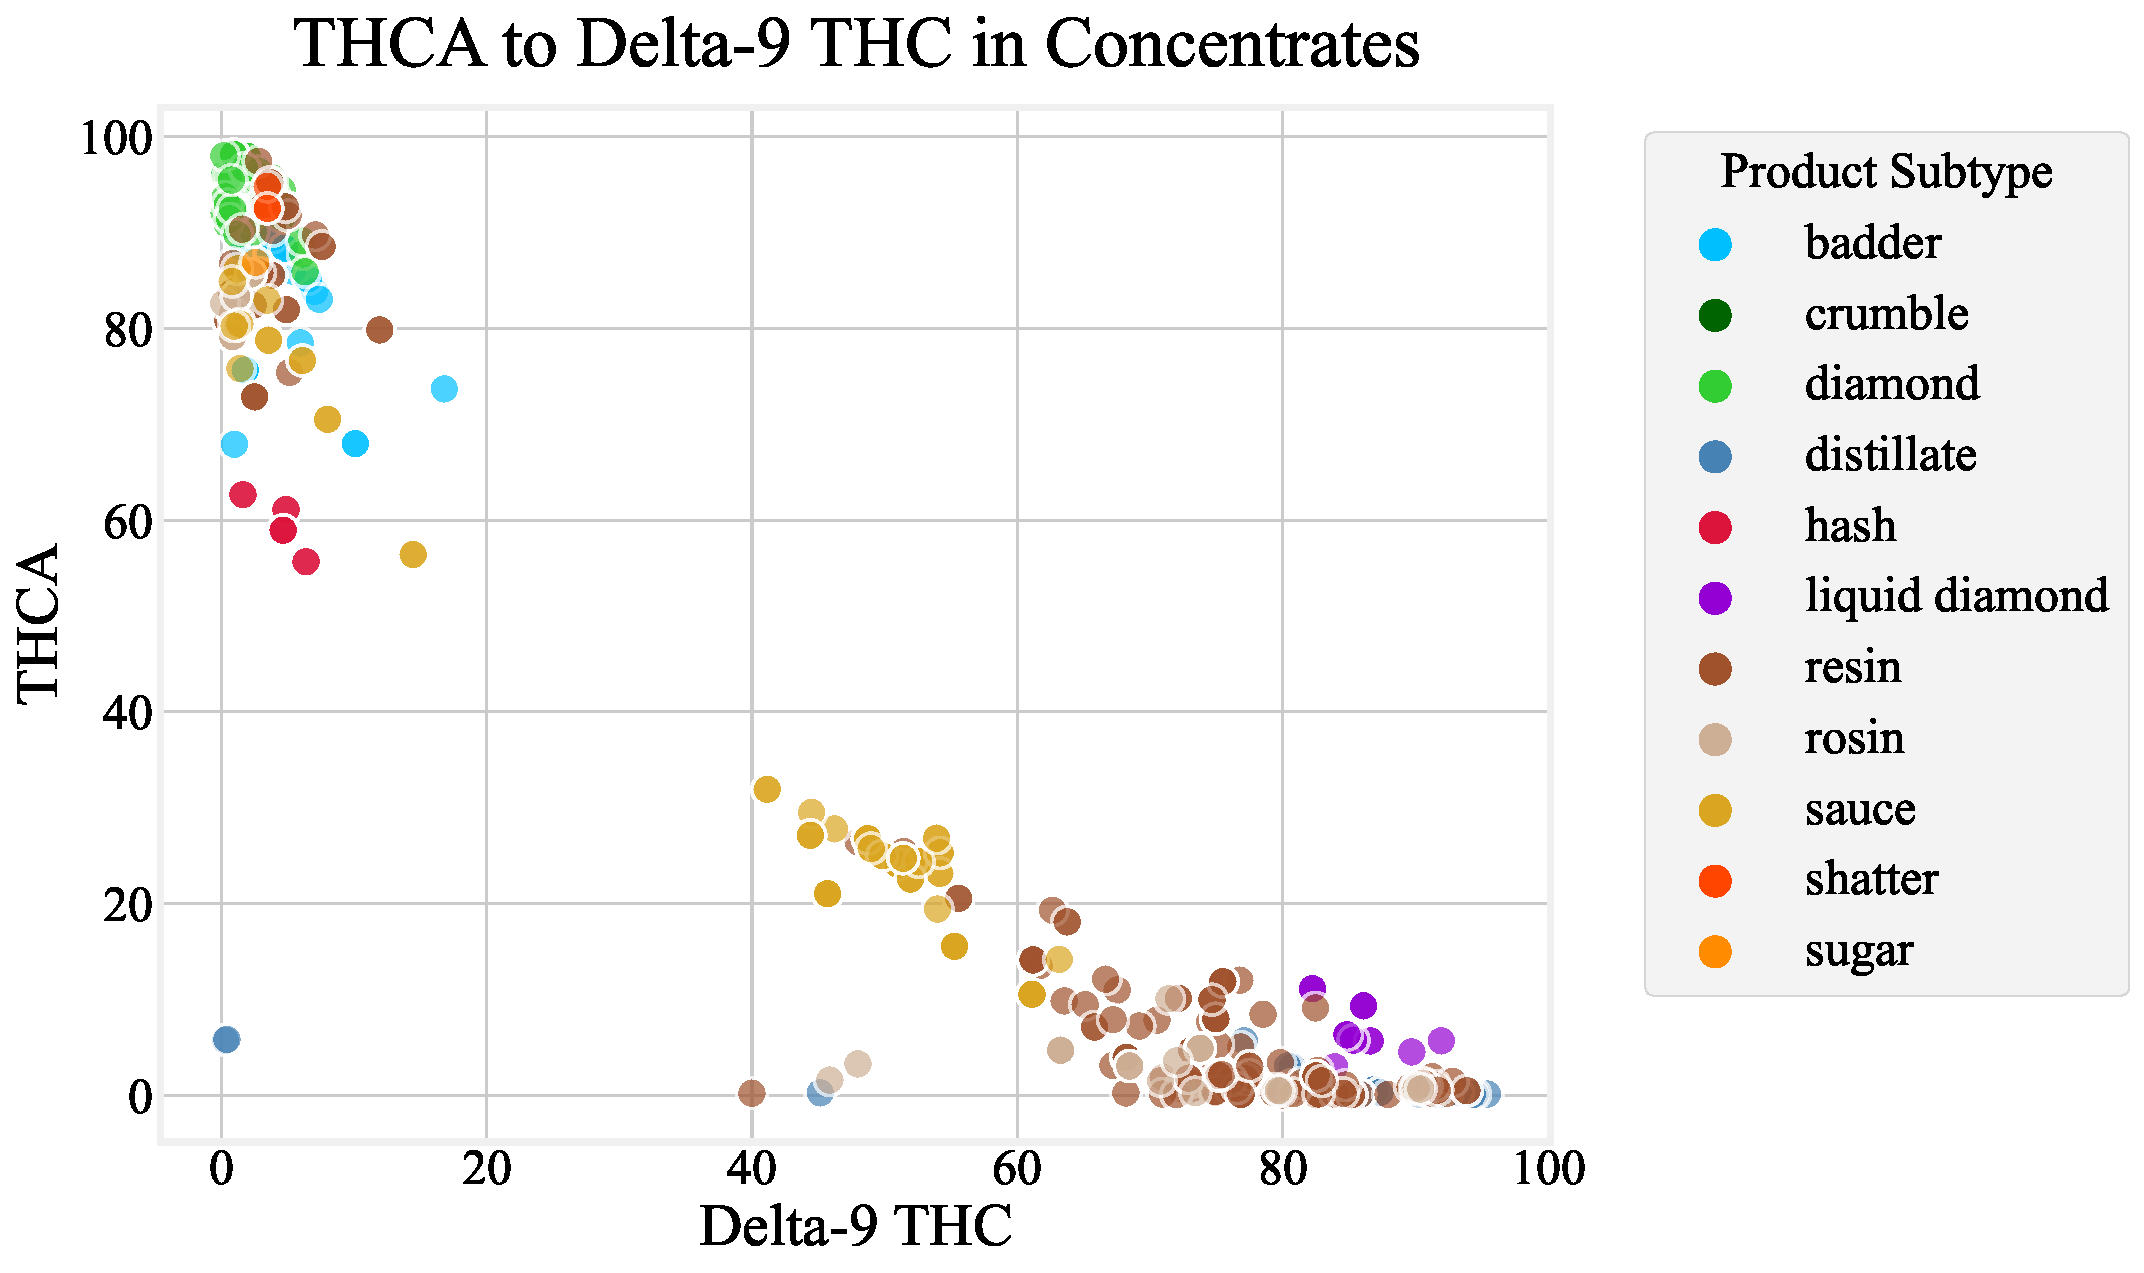
\includegraphics[width=0.8\linewidth]{figures/thca-to-delta-9-thc-concentrates.pdf}
\end{center}


%---------------------------------%
% Cannabinoid Analysis
%---------------------------------%
\newpage

In addition to the major cannabinoids, we also visualize the average concentrations of minor cannabinoids by product category.

\vspace{2\baselineskip}

% Major cannabinoids
\begin{center}
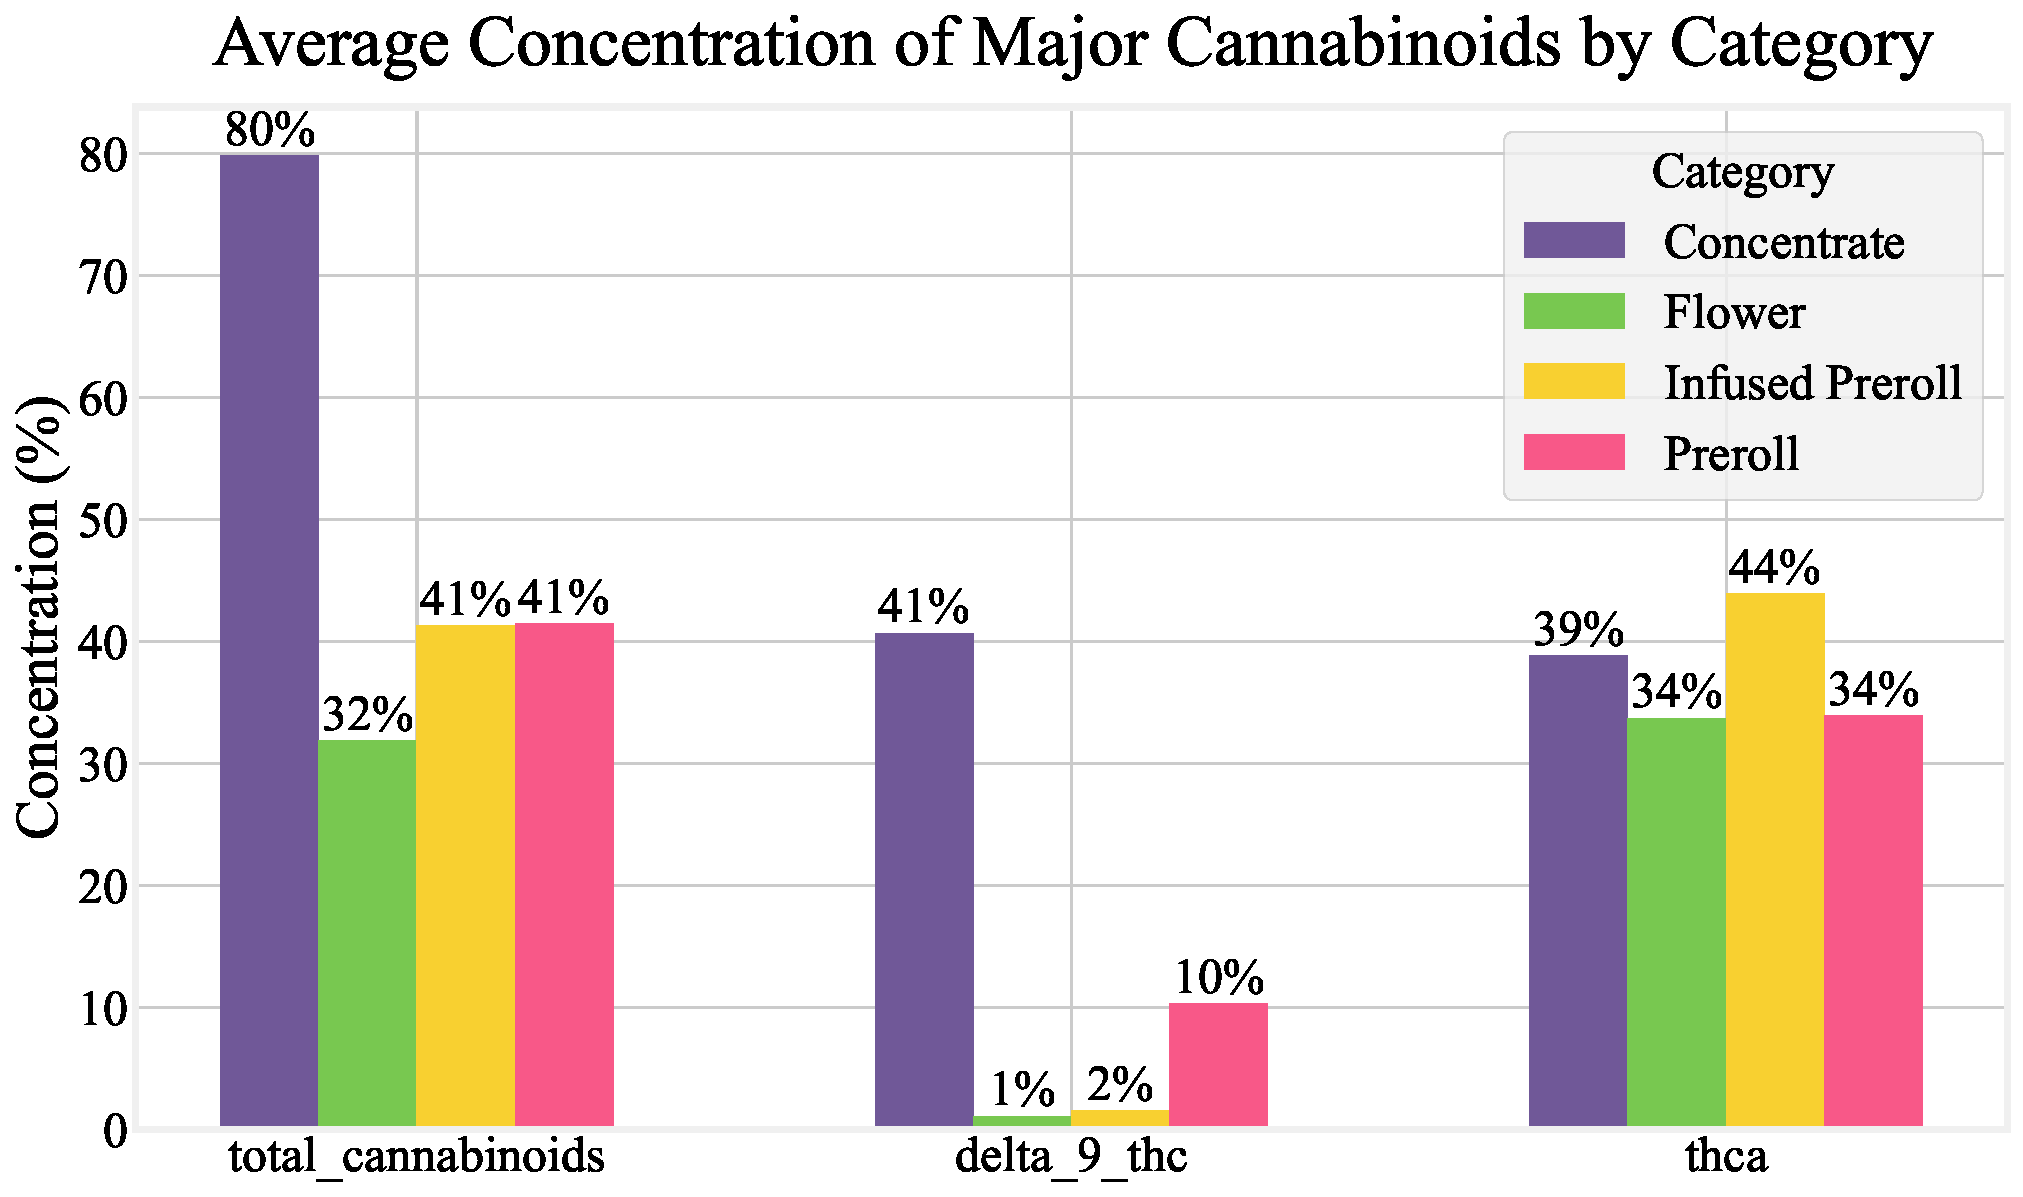
\includegraphics[width=0.8\linewidth]{figures/major-cannabinoids-by-product-category.pdf}
\end{center}

\vspace{2\baselineskip}

% Minor cannabinoids
\begin{center}
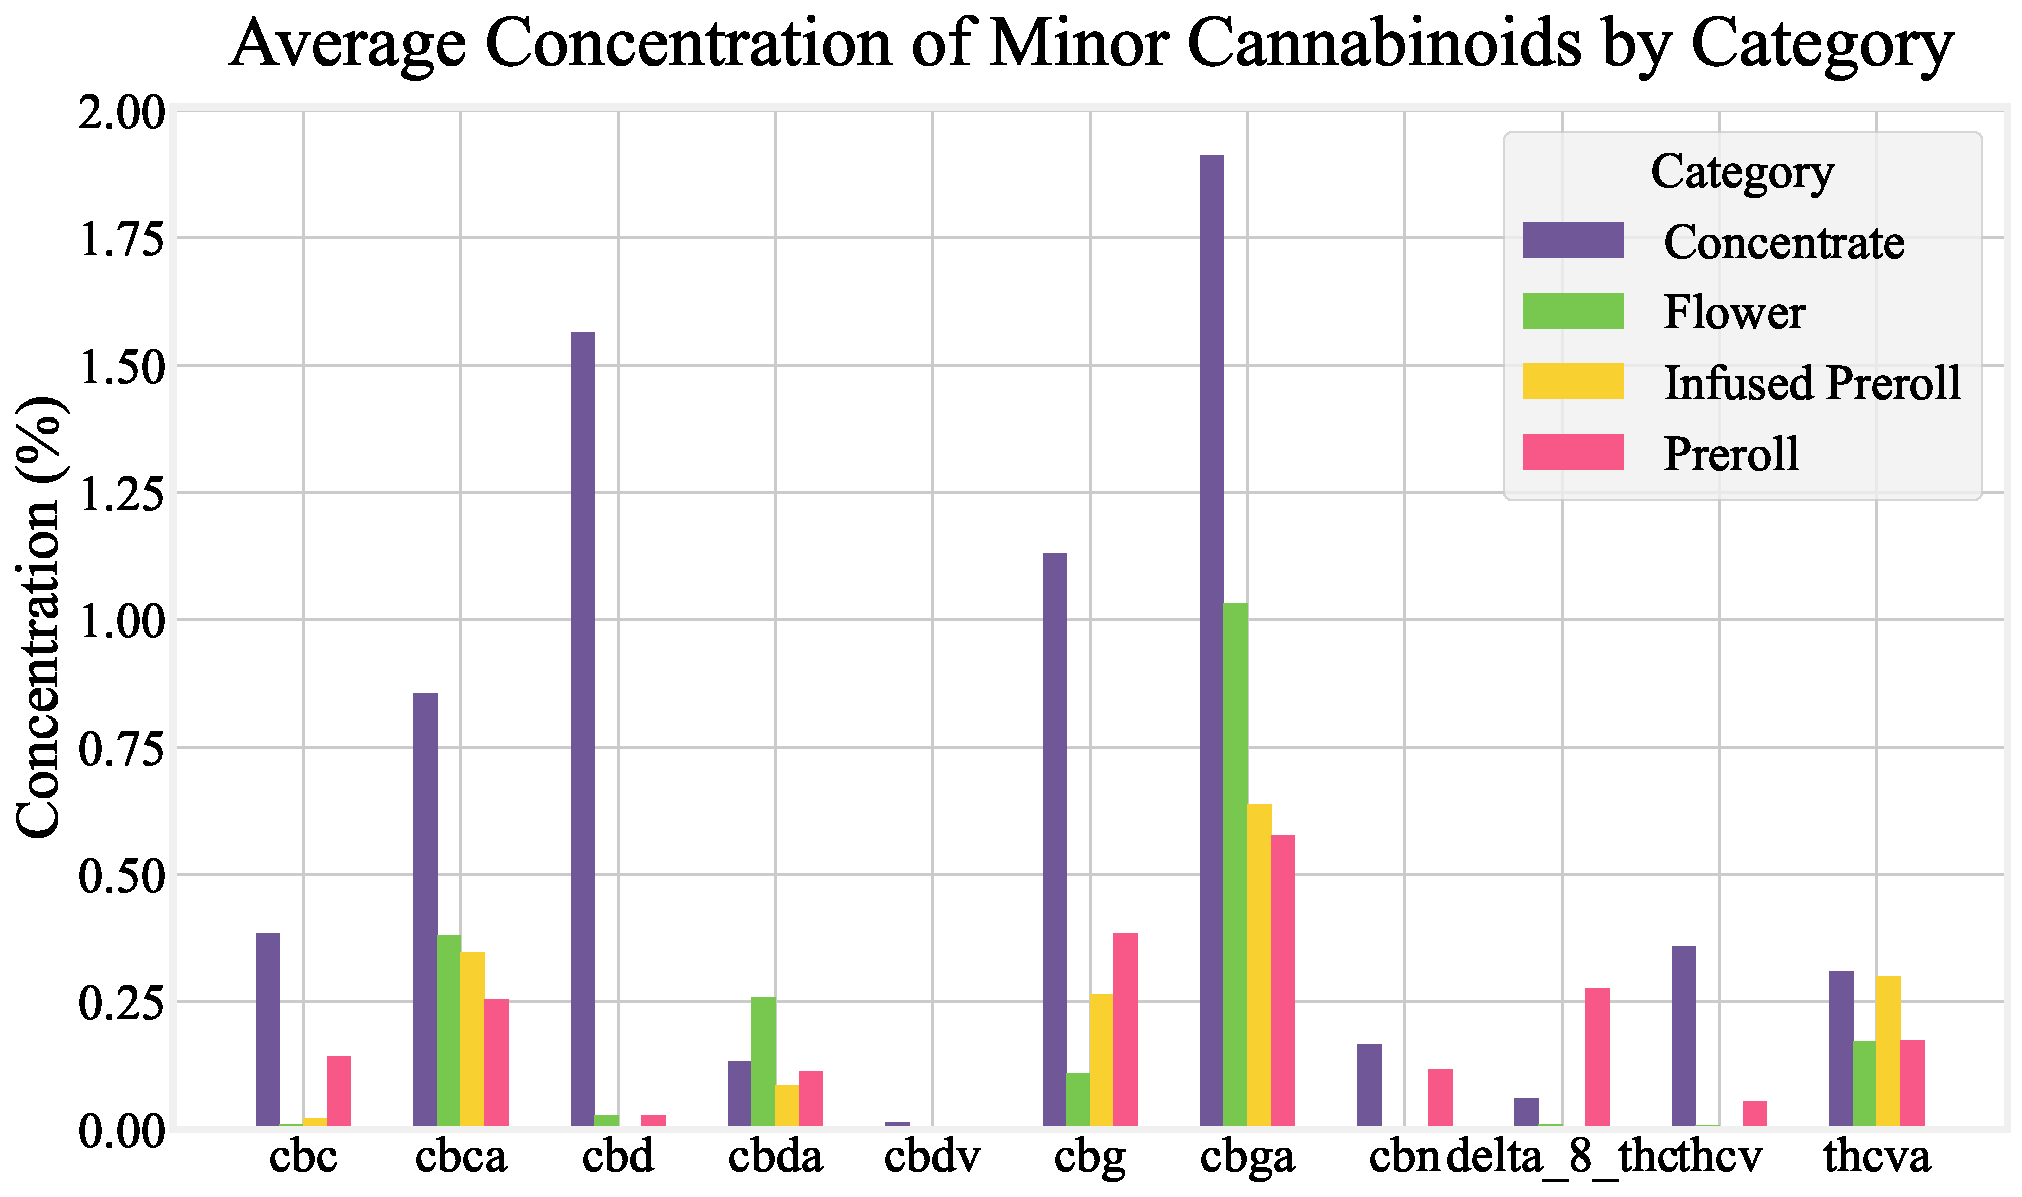
\includegraphics[width=0.8\linewidth]{figures/minor-cannabinoids-by-product-category.pdf}
\end{center}


%---------------------------------%
% Terpene Analysis
%---------------------------------%
\newpage
\section*{Terpene Analysis}
\label{sec:Terpene Analysis}

We turn our eyes now to total terpenes in flower, pre-rolls, and concentrates.

\vspace{1\baselineskip}

% Total terpenes histogram
\begin{center}
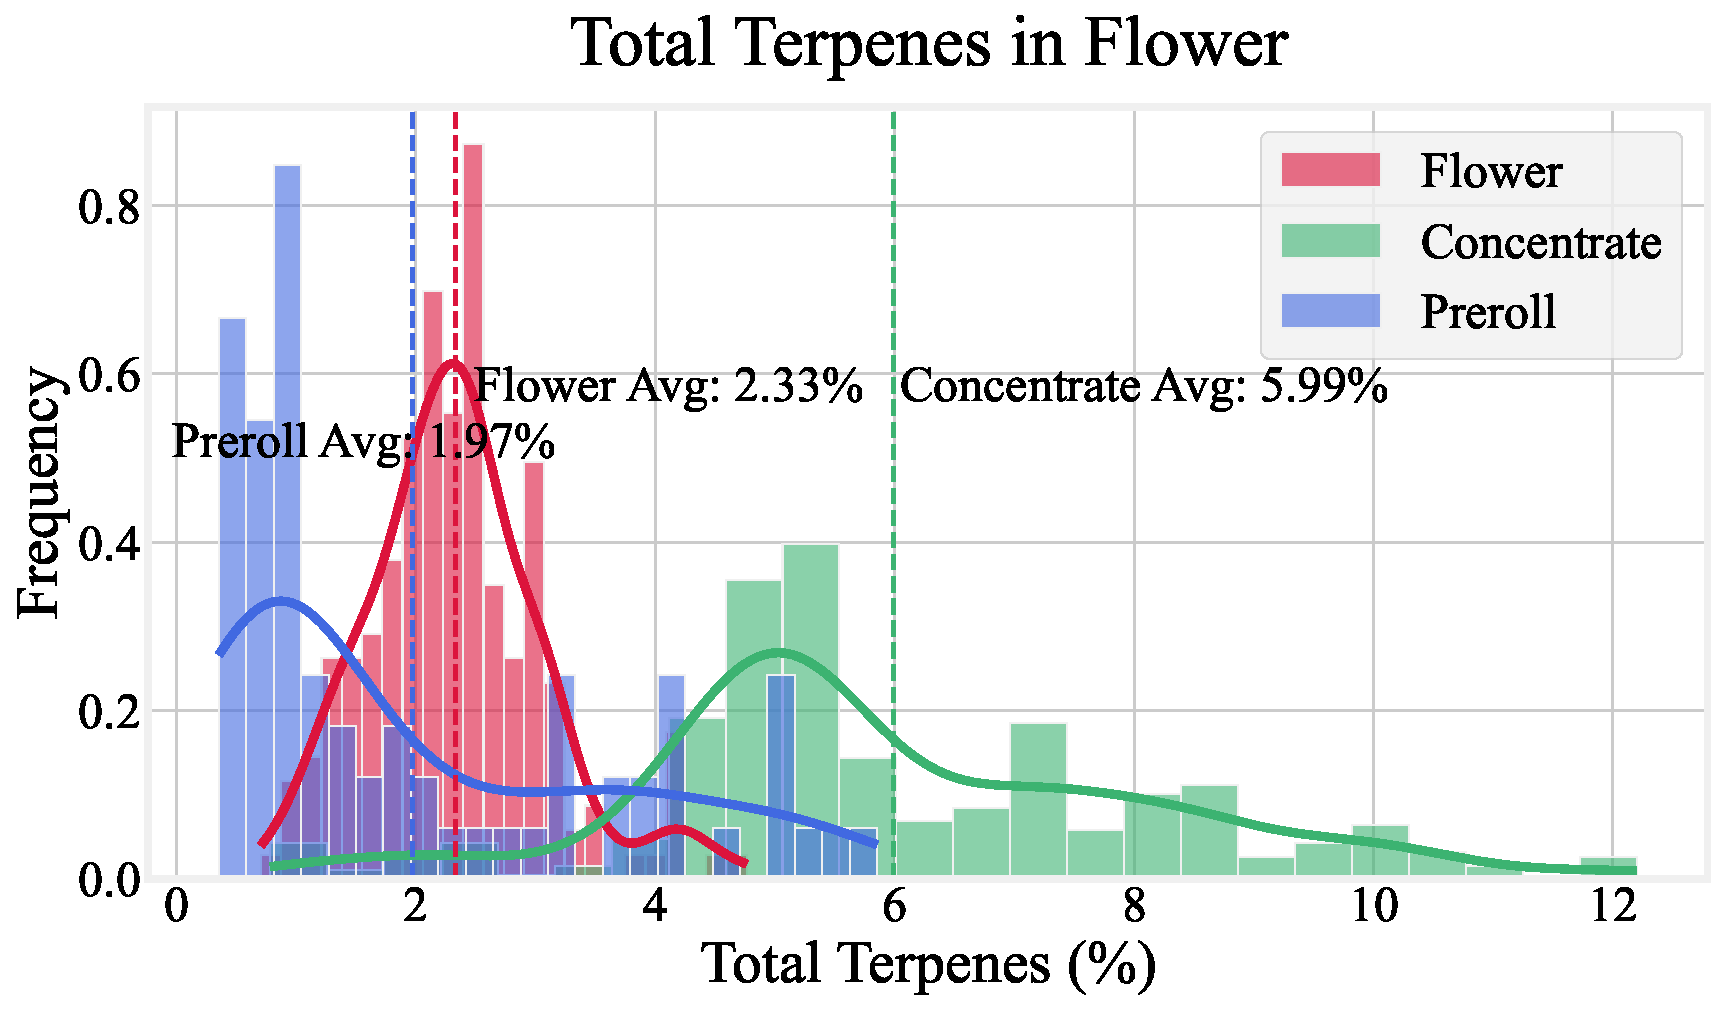
\includegraphics[width=0.8\linewidth]{figures/total-terpenes-histogram.pdf}
\end{center}

\vspace{1\baselineskip}

Here we visualize the average terpene concentrations by product category.

\vspace{2\baselineskip}

% Terpene profile
\begin{center}
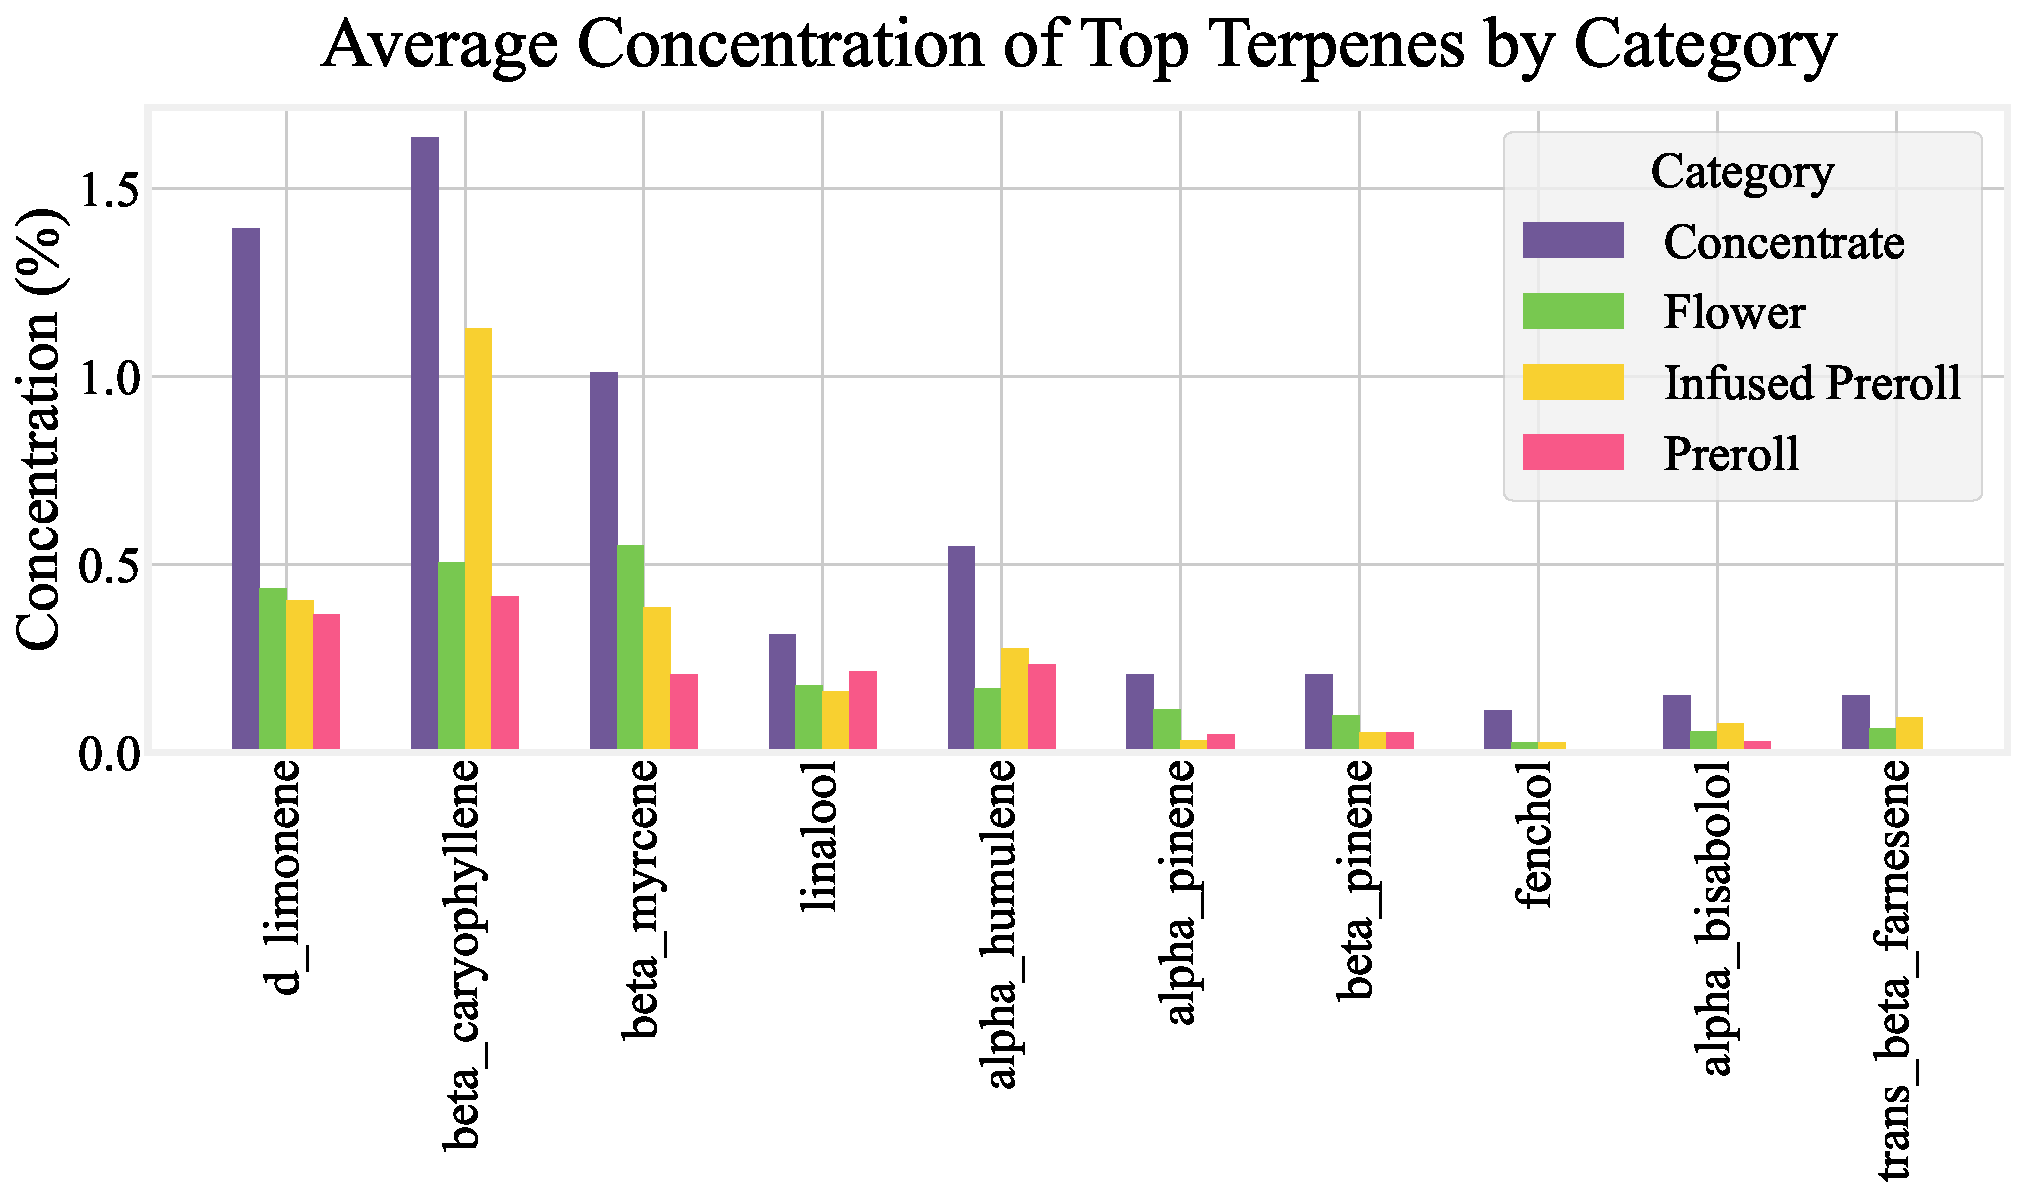
\includegraphics[width=0.8\linewidth]{figures/top-terpenes-by-product-category.pdf}
\end{center}

\newpage

We also look at the prevelance of dominant terpenes by category.

\vspace{1\baselineskip}

% Dominant terpenes by category
\begin{center}
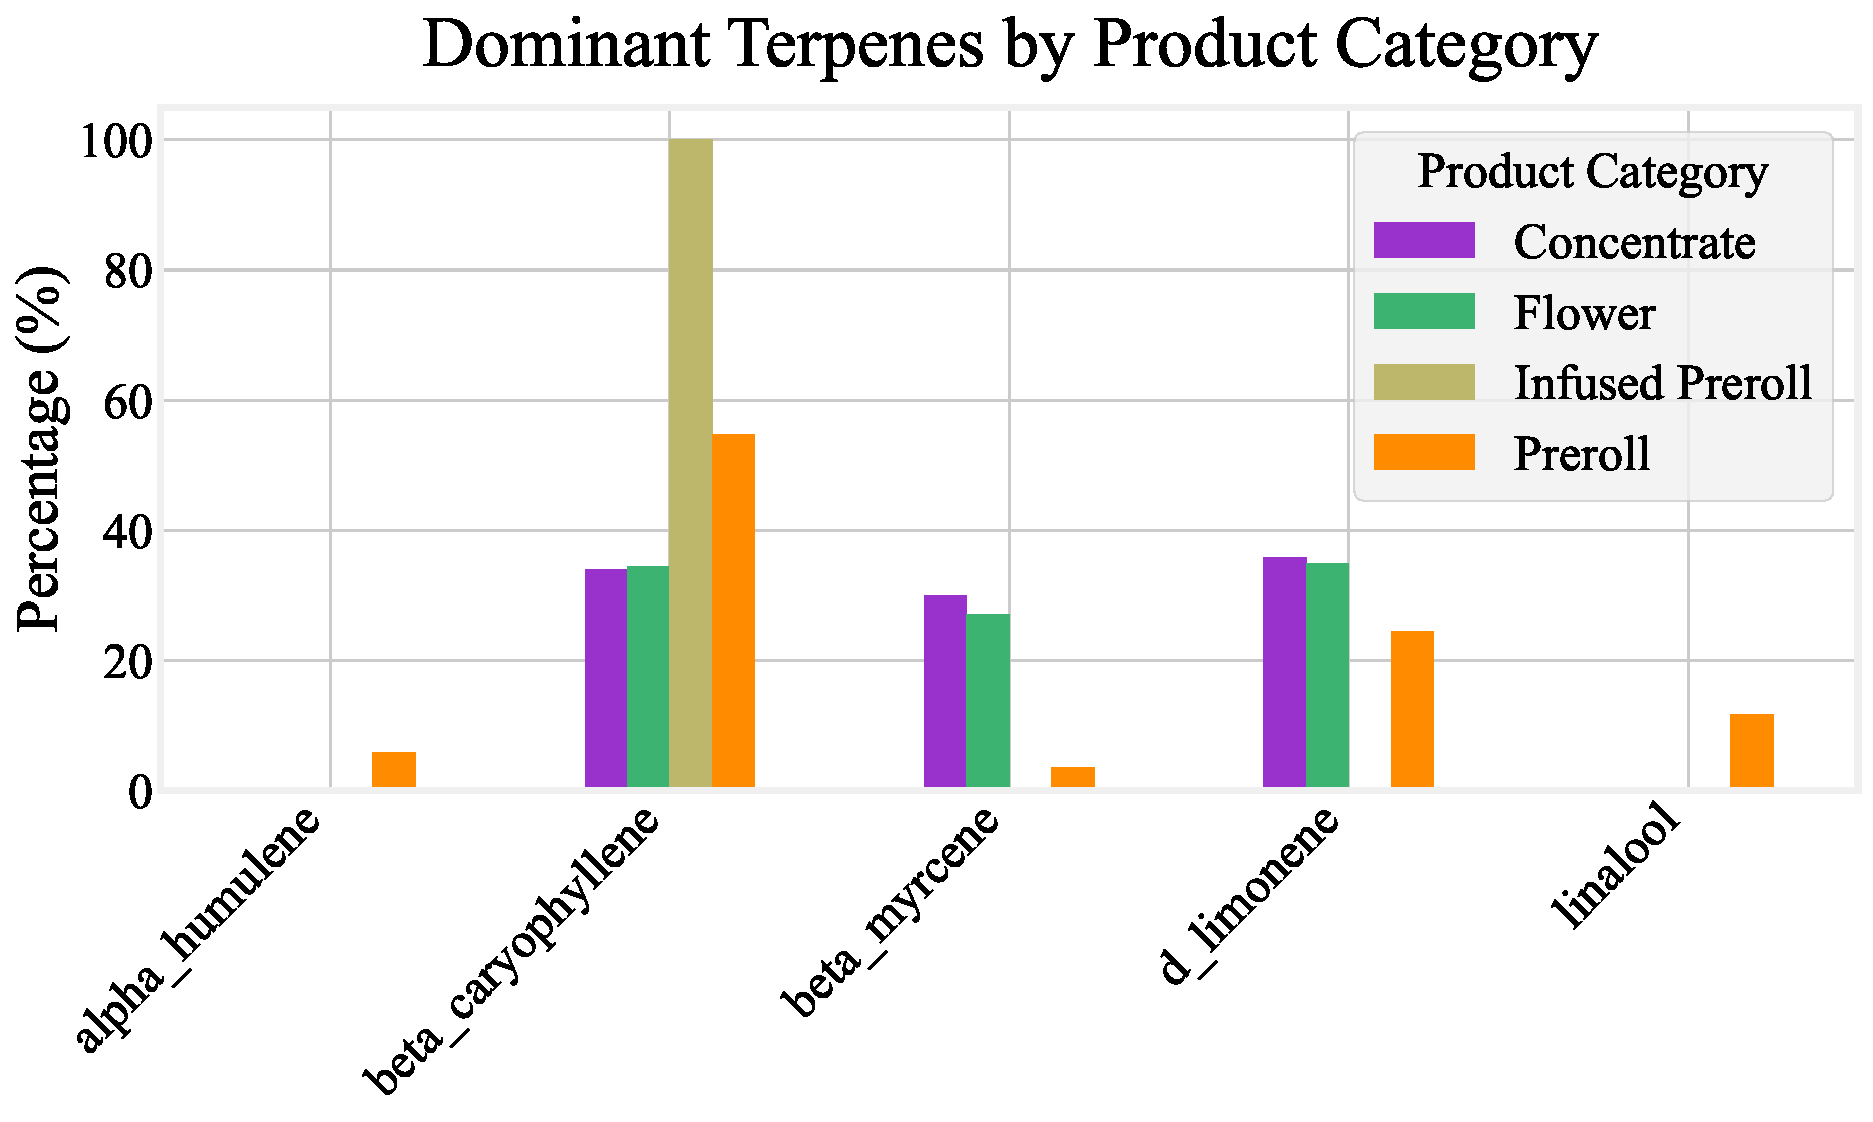
\includegraphics[width=0.6\linewidth]{figures/dominant-terpenes-by-category.pdf}
\end{center}

\vspace{1\baselineskip}

We can also visualize ratios of terpenes that are highly correlated.

\vspace{0.5\baselineskip}

% alpha-humulene to beta-caryophyllene
\begin{center}
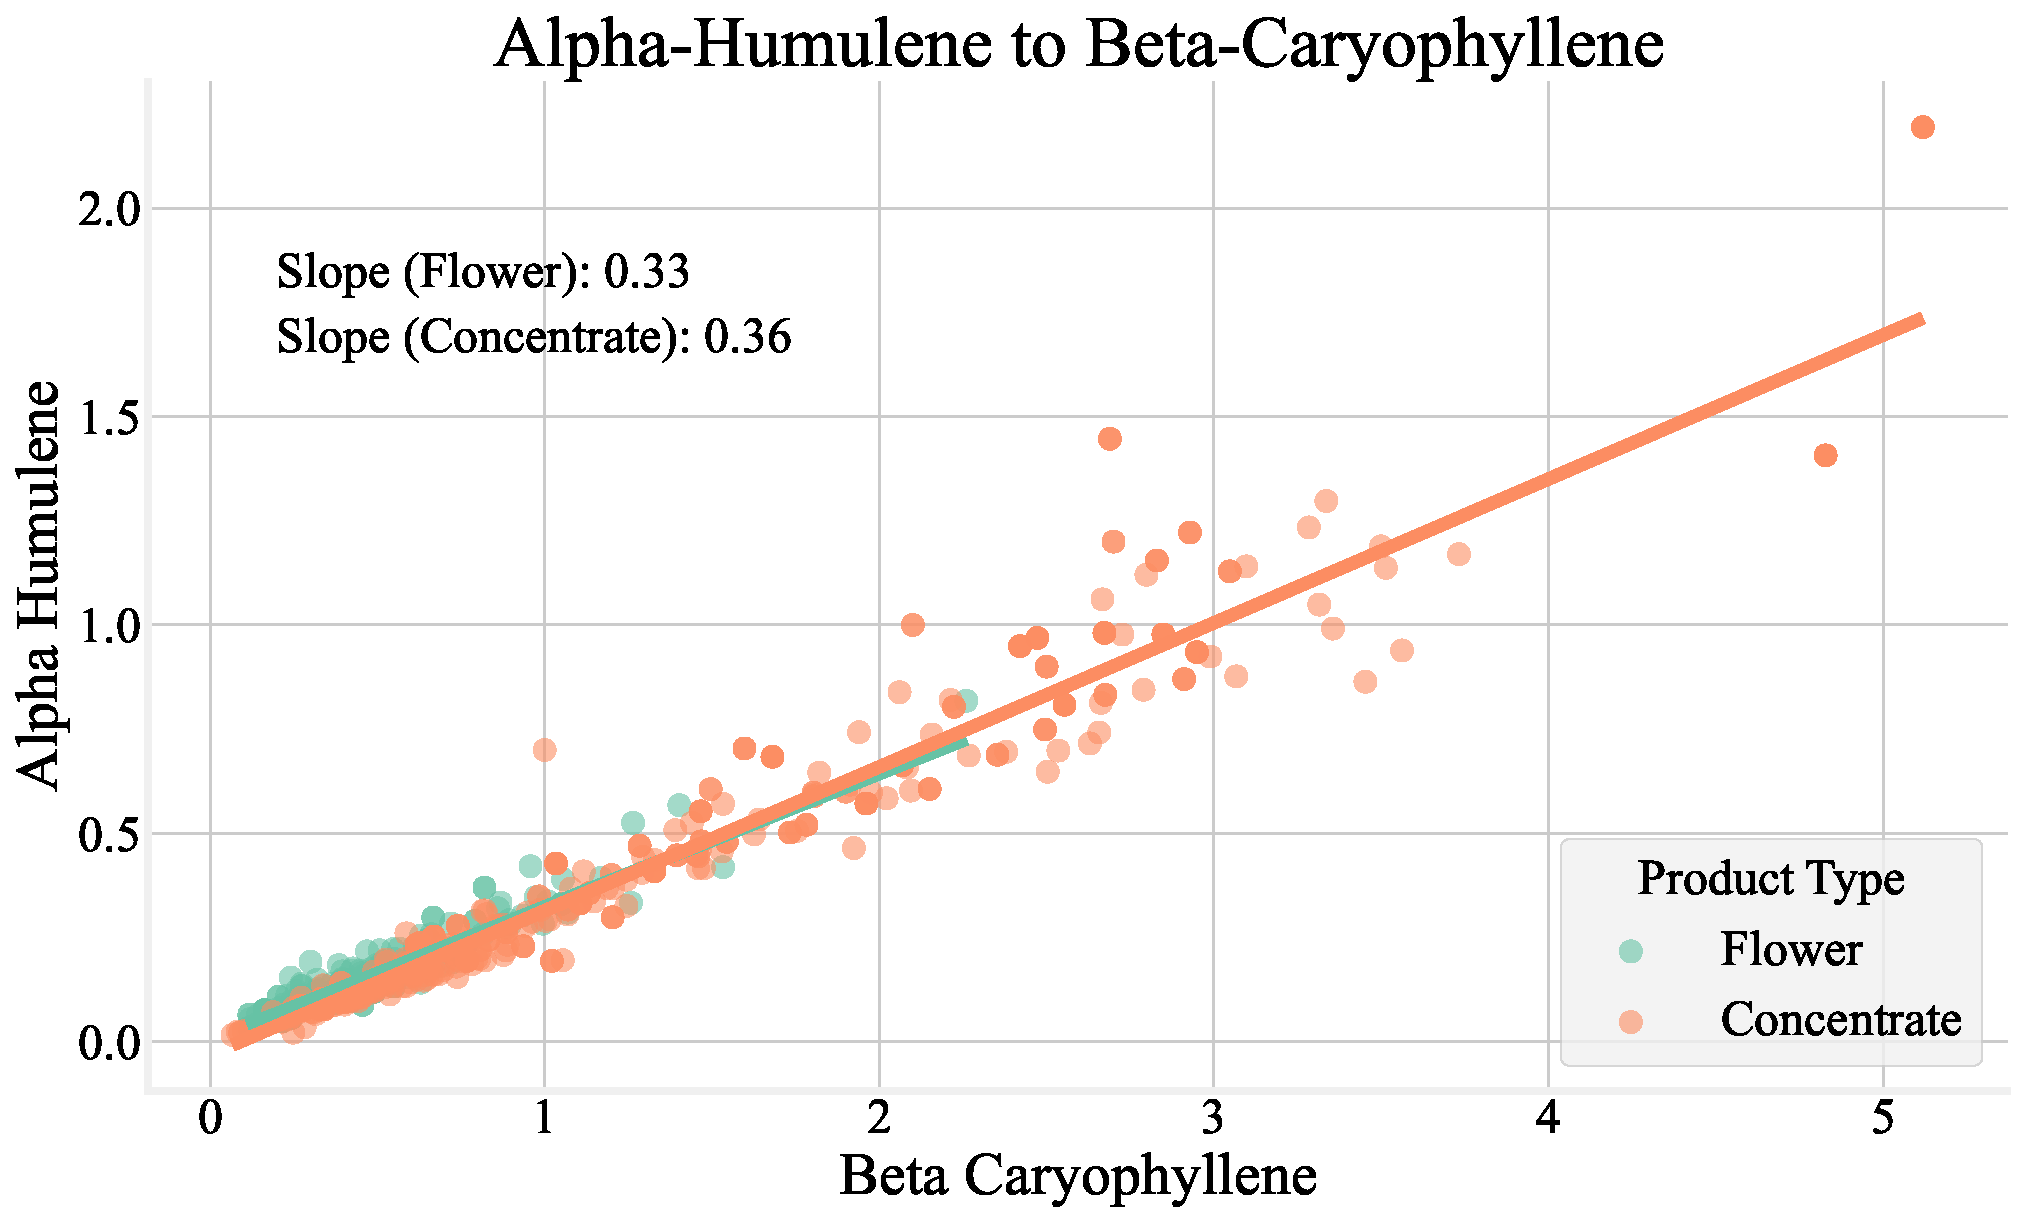
\includegraphics[width=0.55\linewidth]{figures/alpha-humulene-to-beta-caryophyllene.pdf}
\end{center}

\vspace{0.5\baselineskip}

% camphene to d-limonene
\begin{center}
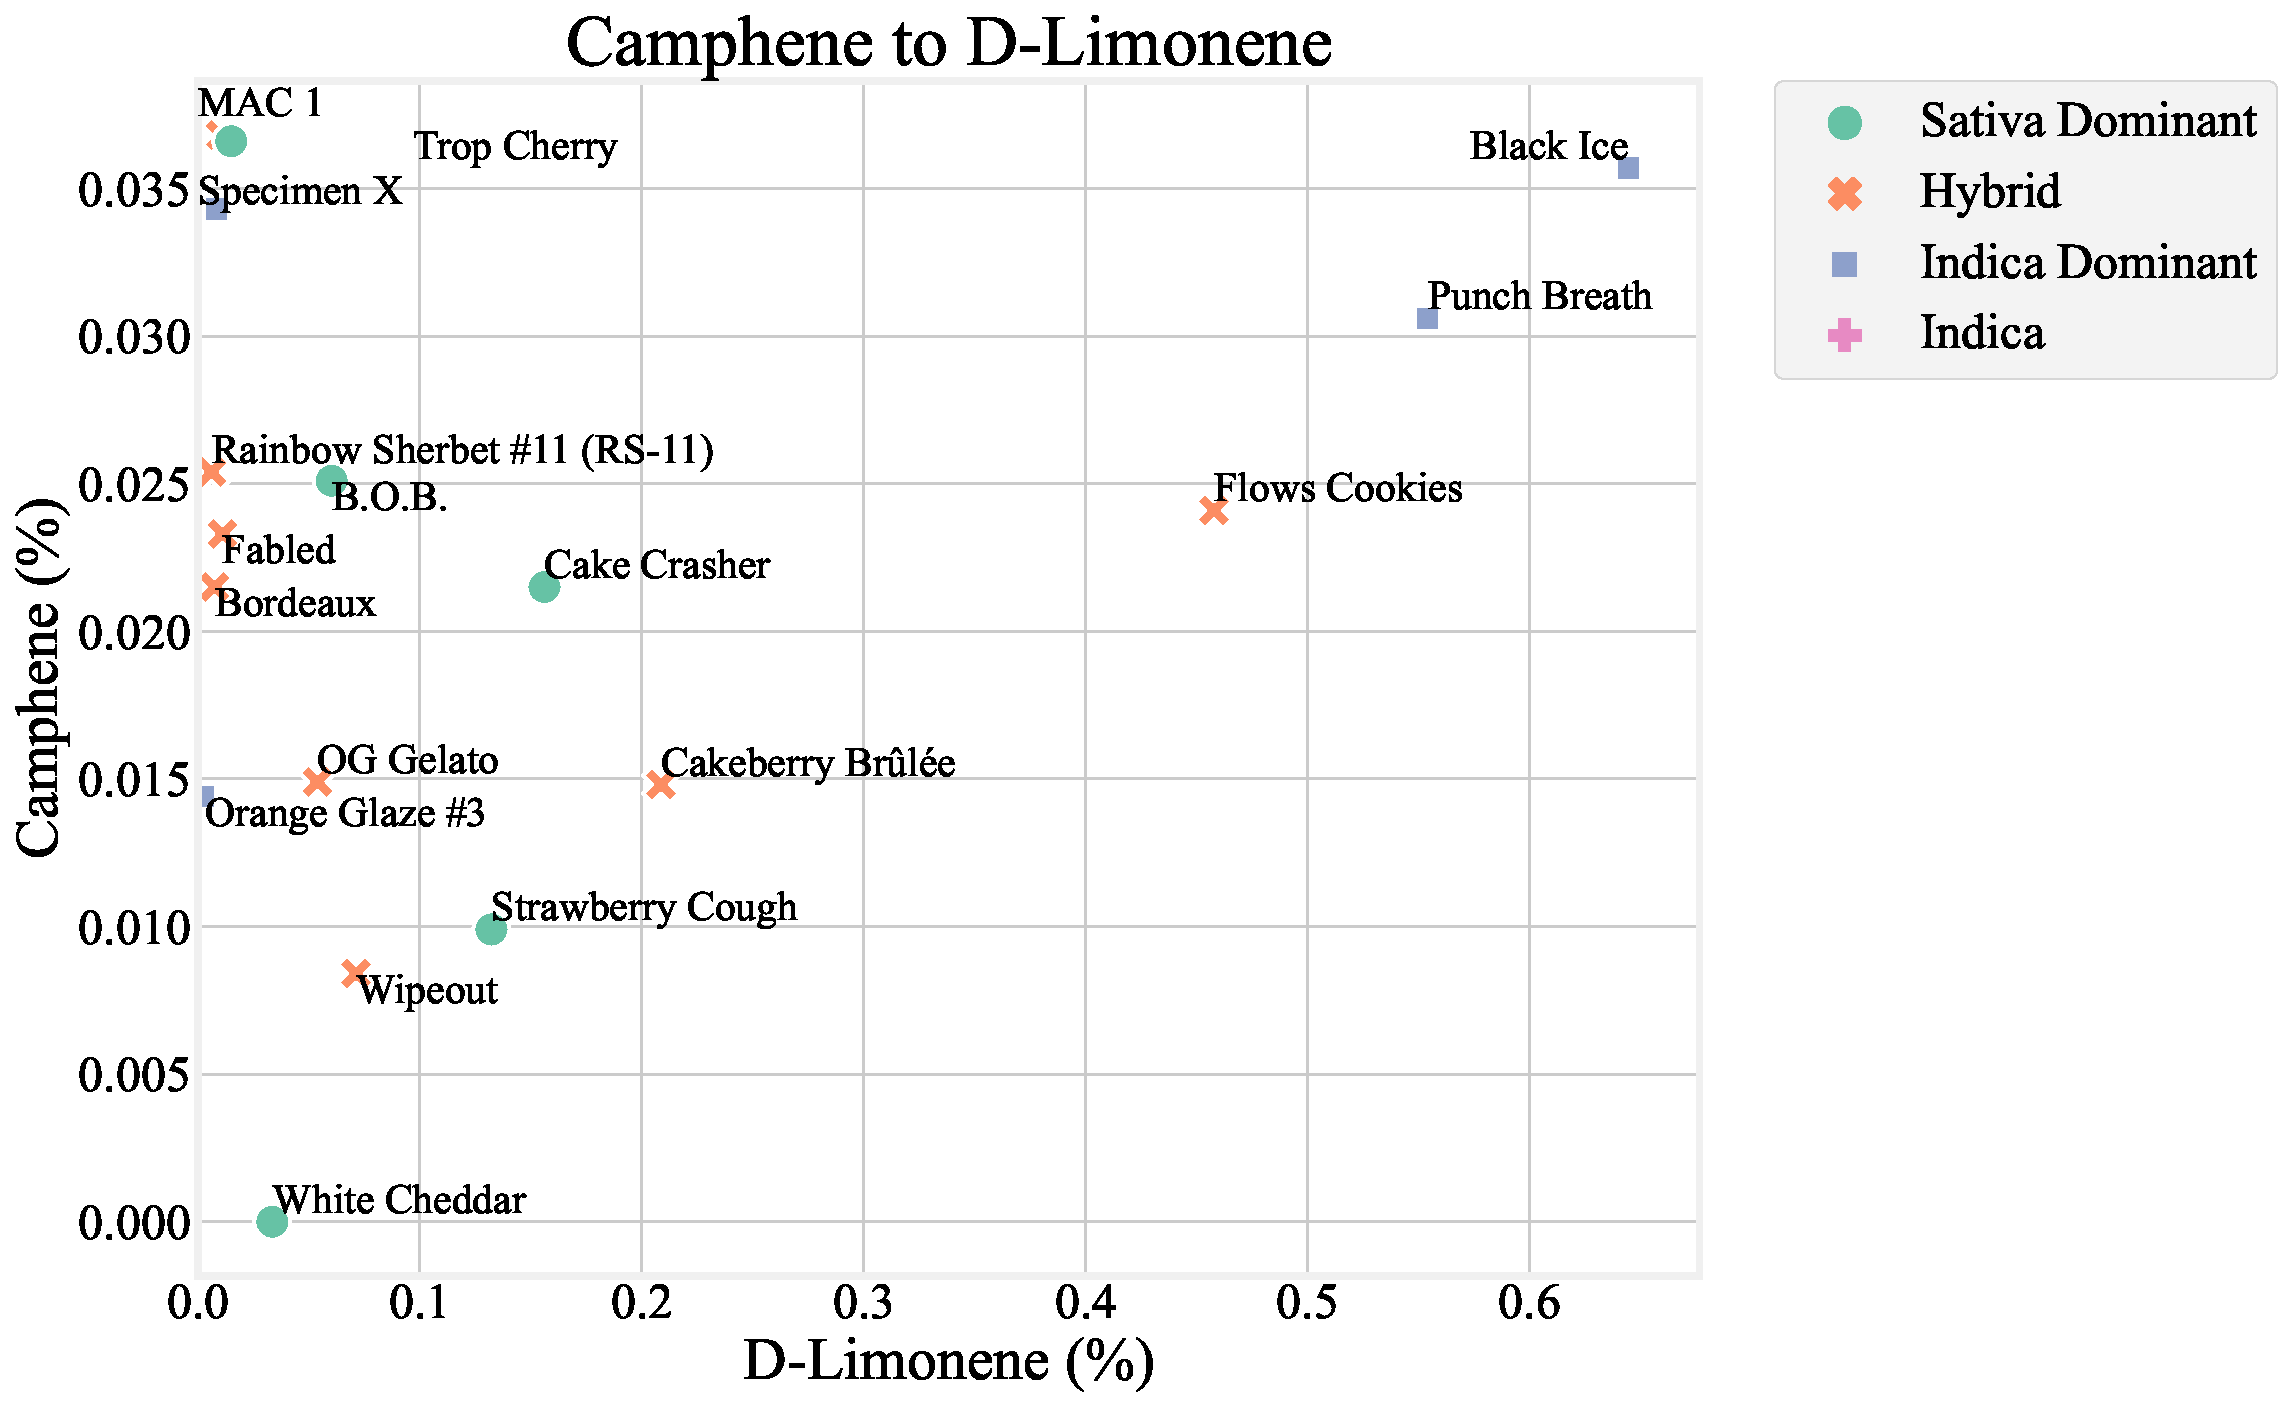
\includegraphics[width=0.55\linewidth]{figures/camphene-to-d-limonene.pdf}
\end{center}

\newpage
Here we use a principal component analysis (PCA) of major terpenes to visualize how lab results cluster by dominant terpene, lab, and producer.

\vspace{2\baselineskip}

{\centering

% PCA dominant terpenes
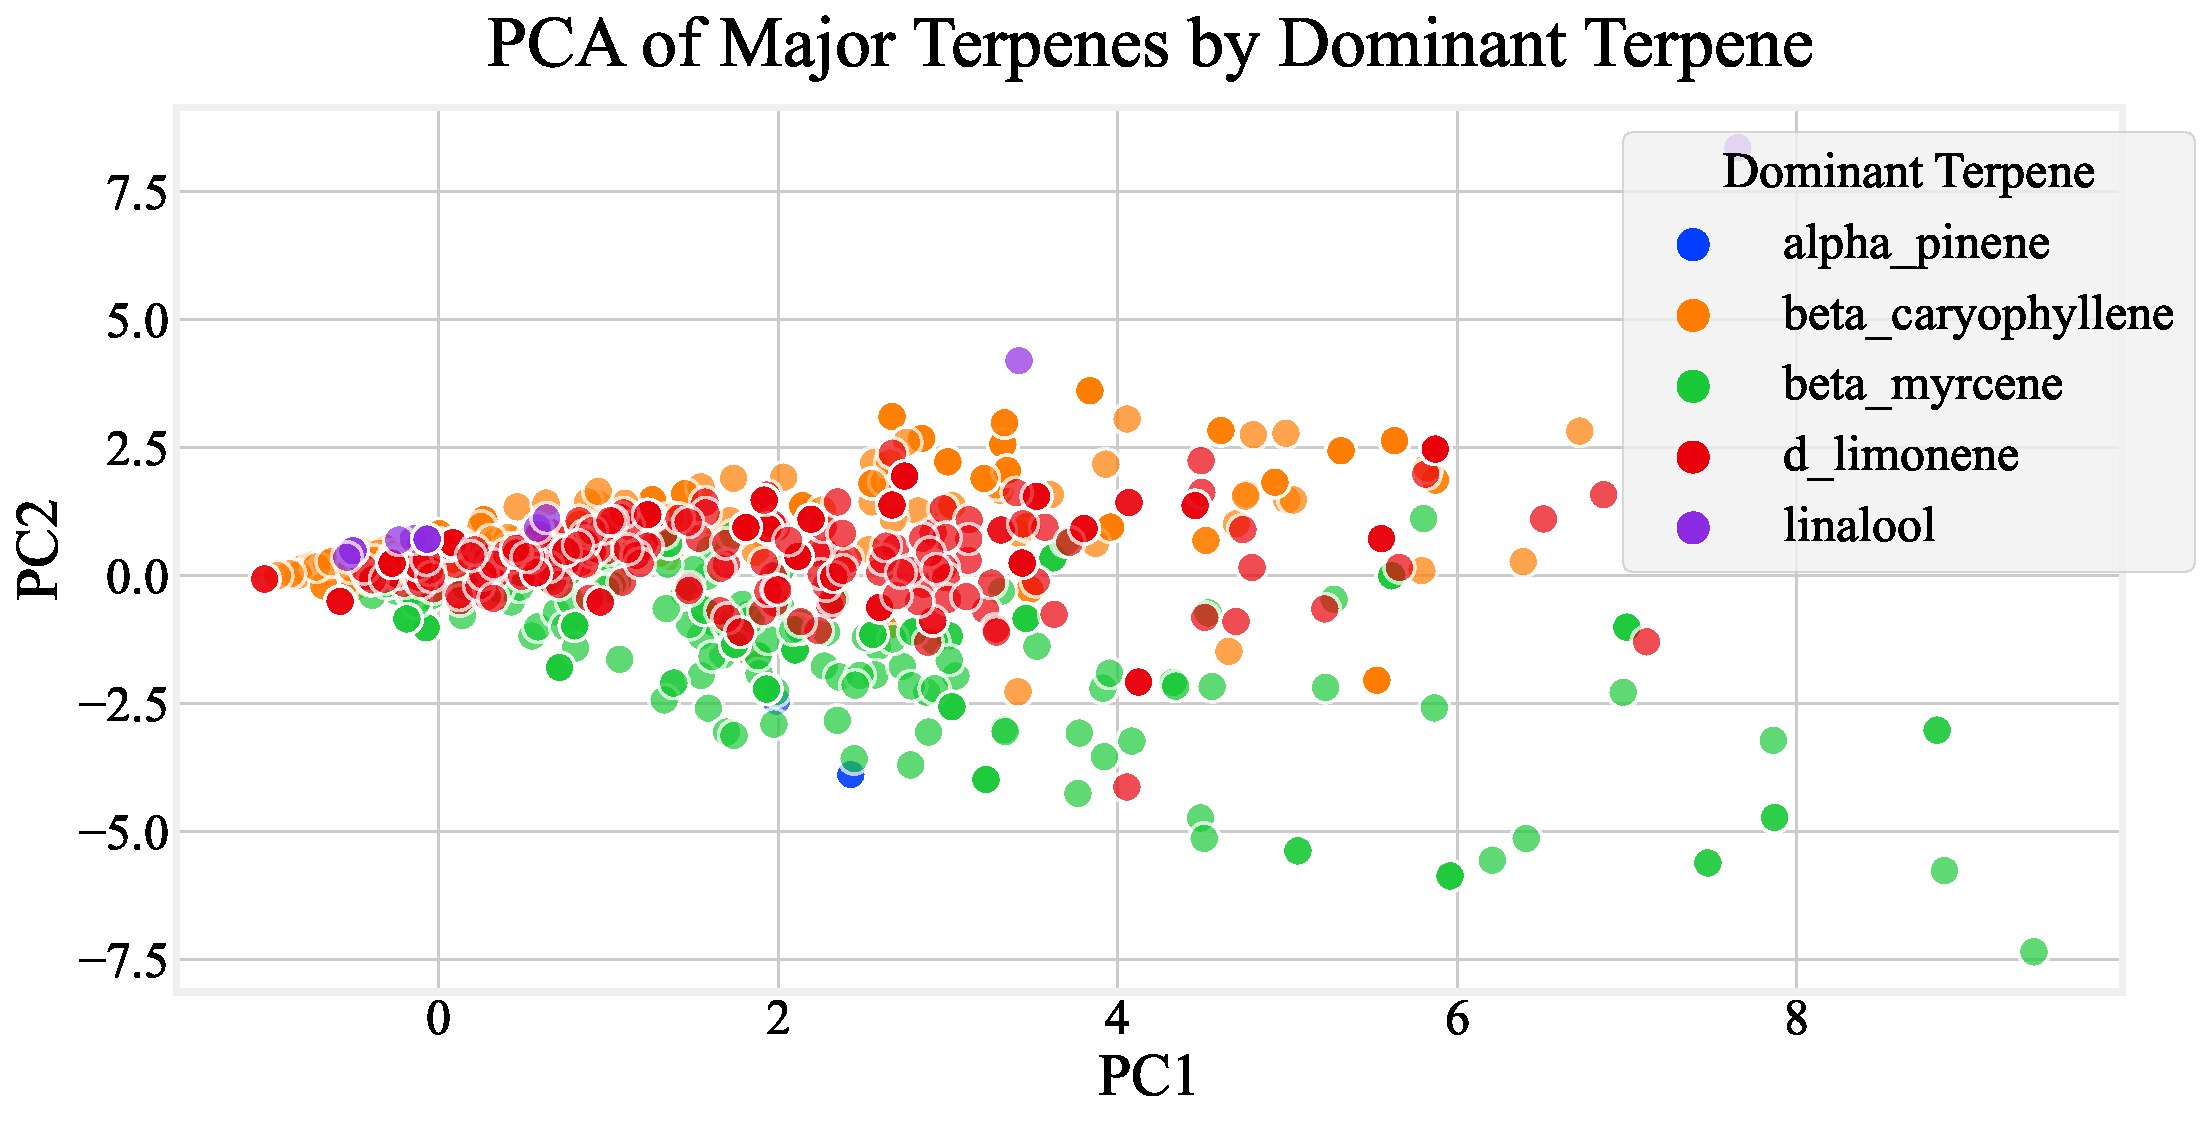
\includegraphics[width=0.7\linewidth]{figures/pca-dominant-terpenes.pdf}

\vspace{1\baselineskip}

% PCA dominant terpenes
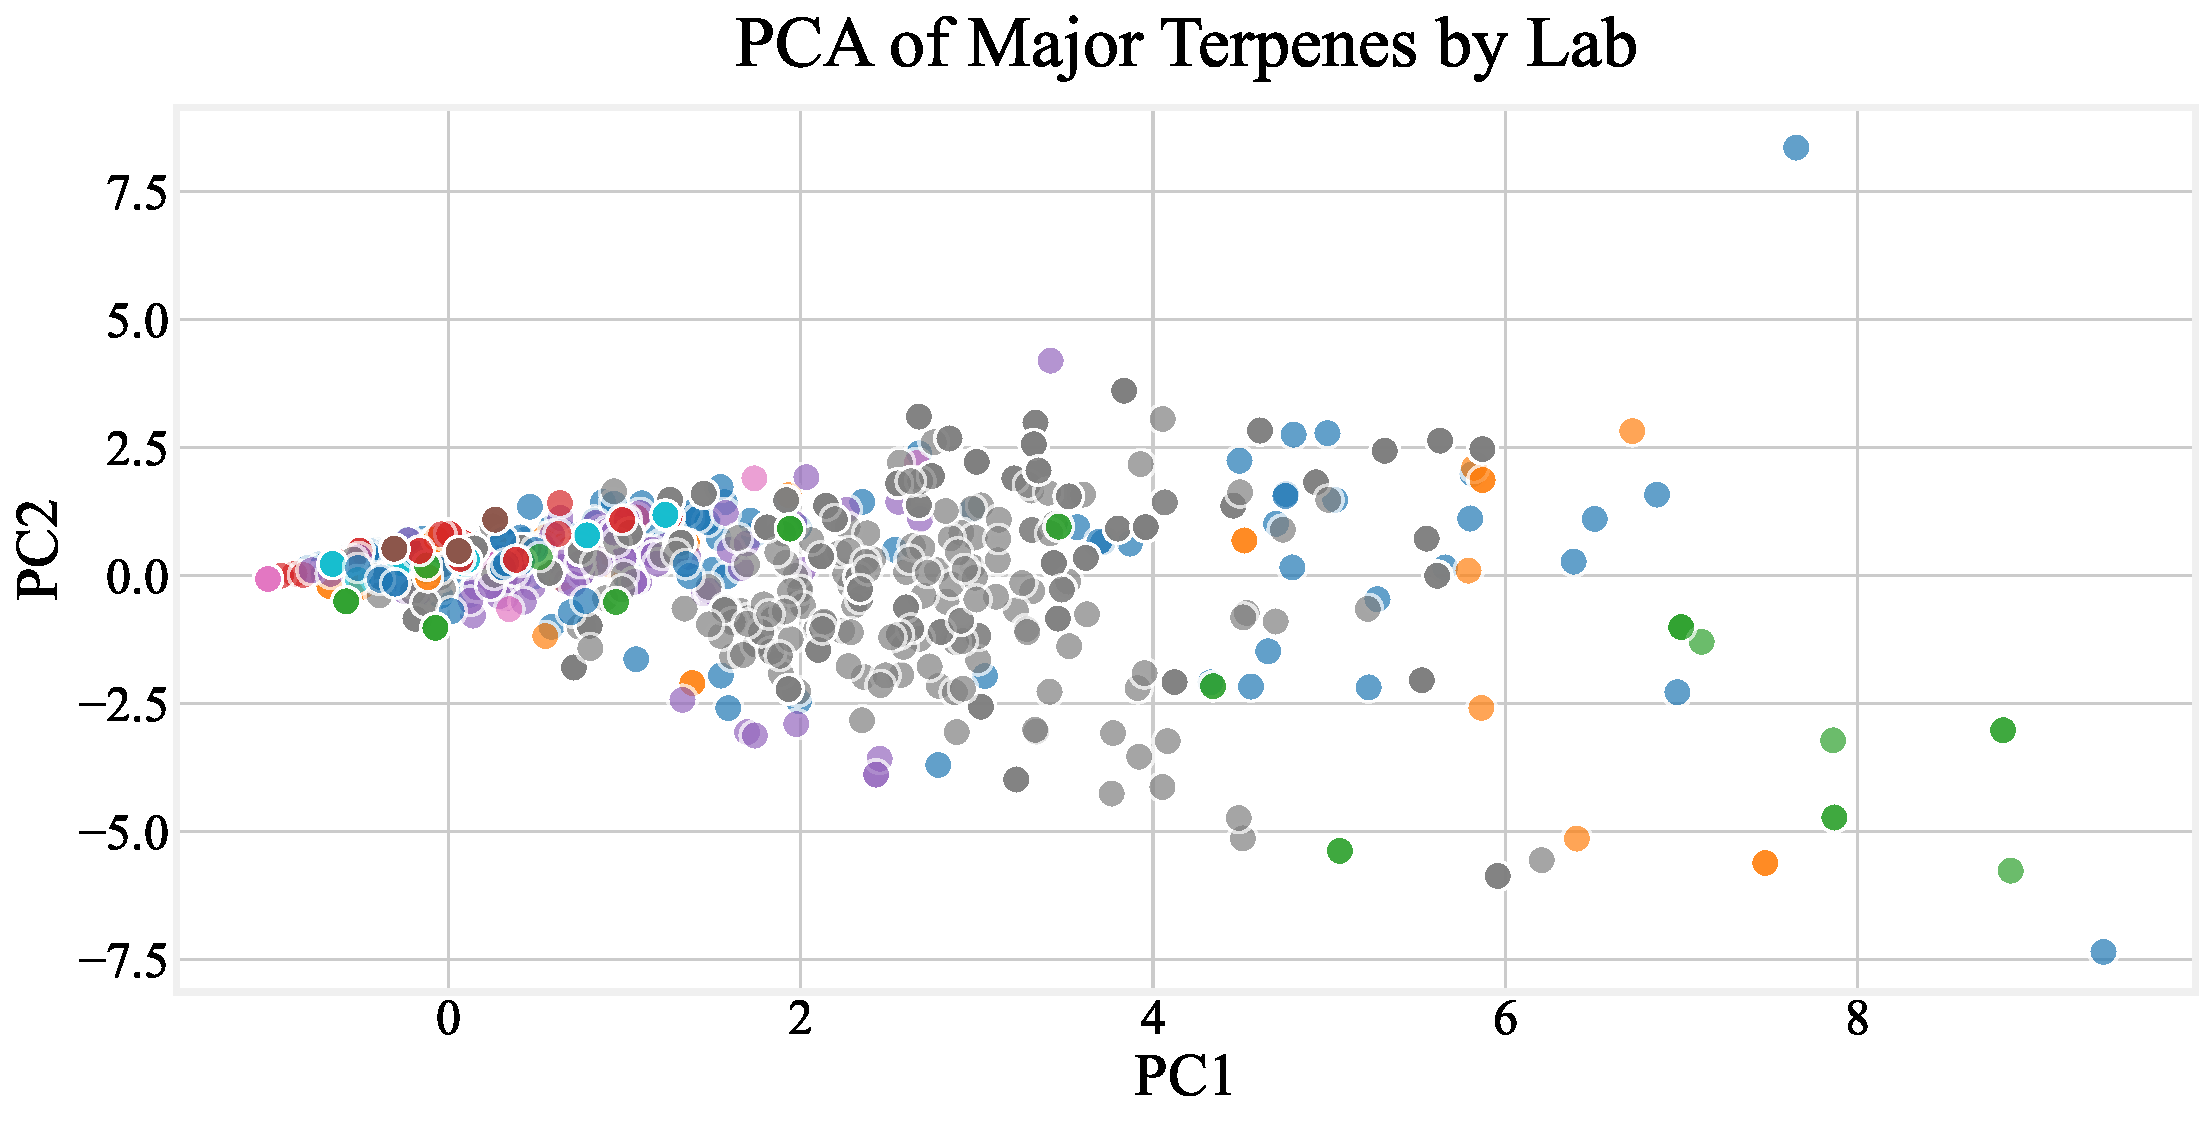
\includegraphics[width=0.7\linewidth]{figures/pca-by-lab.pdf}

\vspace{1\baselineskip}

% PCA dominant terpenes
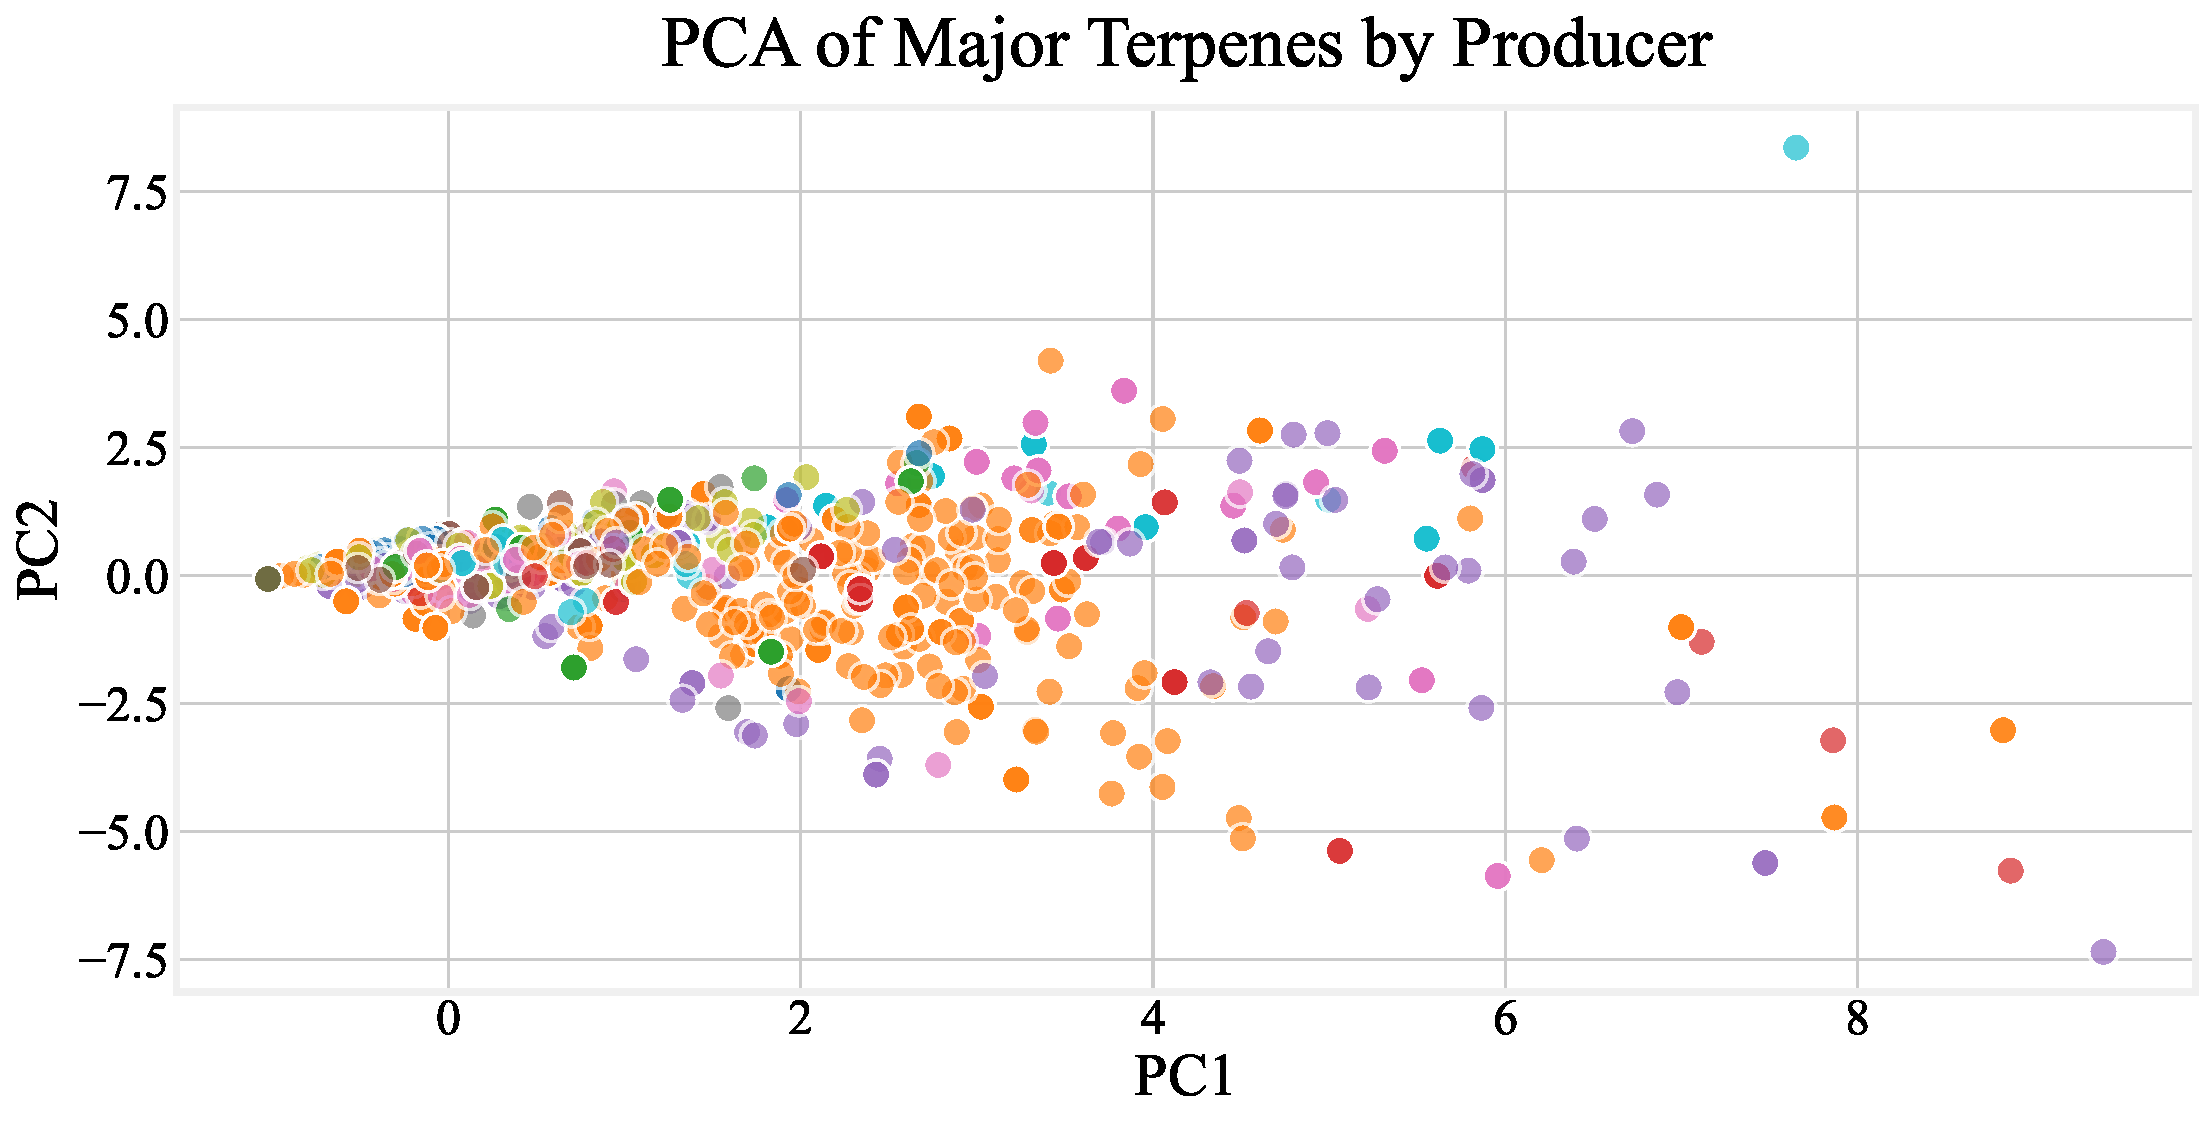
\includegraphics[width=0.7\linewidth]{figures/pca-by-producer.pdf}

}

% OPTIONAL: Detection rates bar chart?


% OPTIONAL: Cannabinoid and terpene diversity.


%---------------------------------%
% Trend Analysis
%---------------------------------%
\newpage
\section*{Trend Analysis}
\label{sec:Trend Analysis}

\vspace{2\baselineskip}

% Total Cannabinoids Flower timeseries
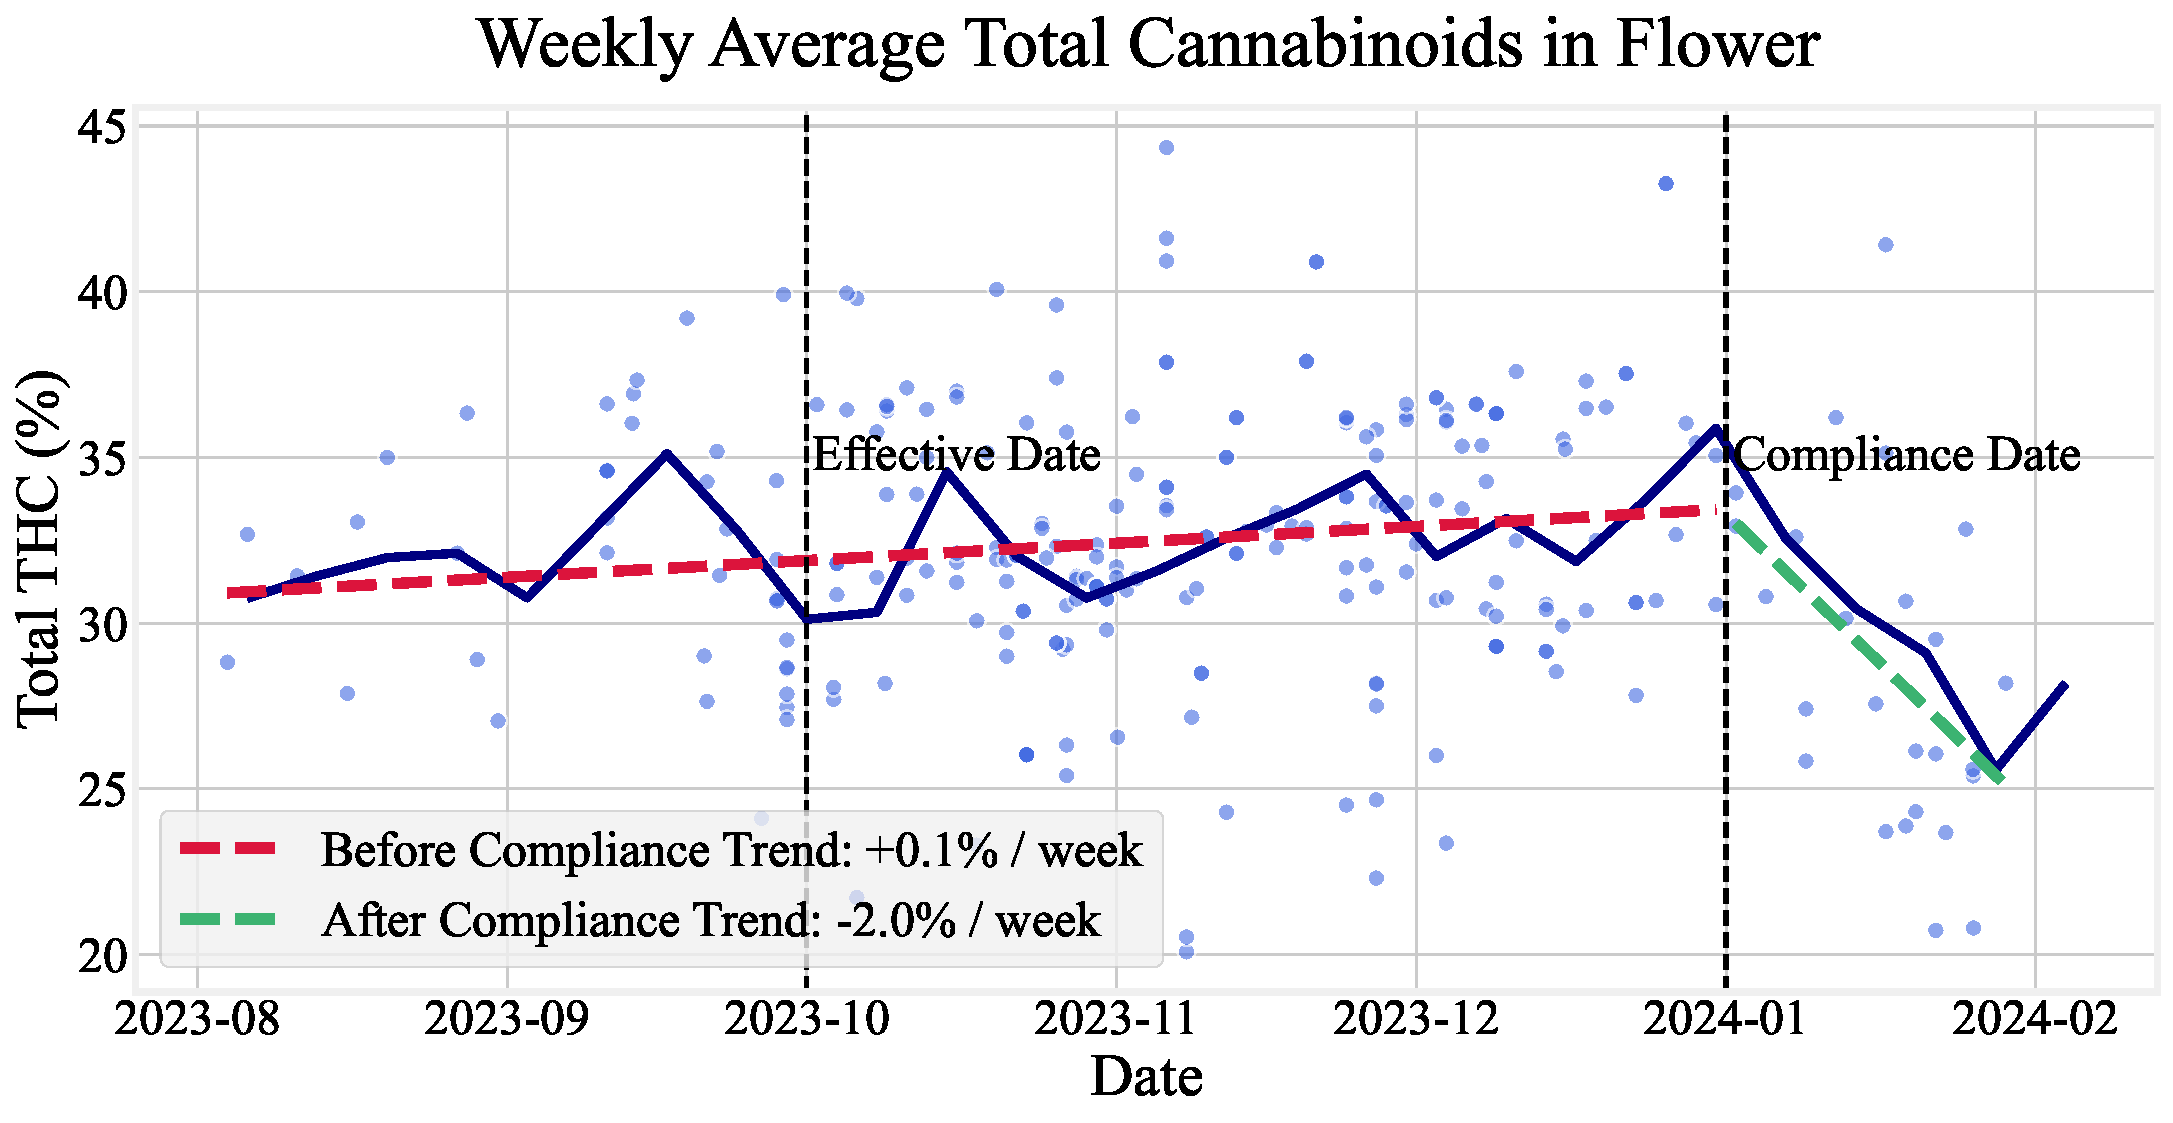
\includegraphics[width=\linewidth]{figures/total-cannabinoids-flower-timeseries.pdf}

\vspace{2\baselineskip}

% Total Cannabinoids Concentrates timeseries
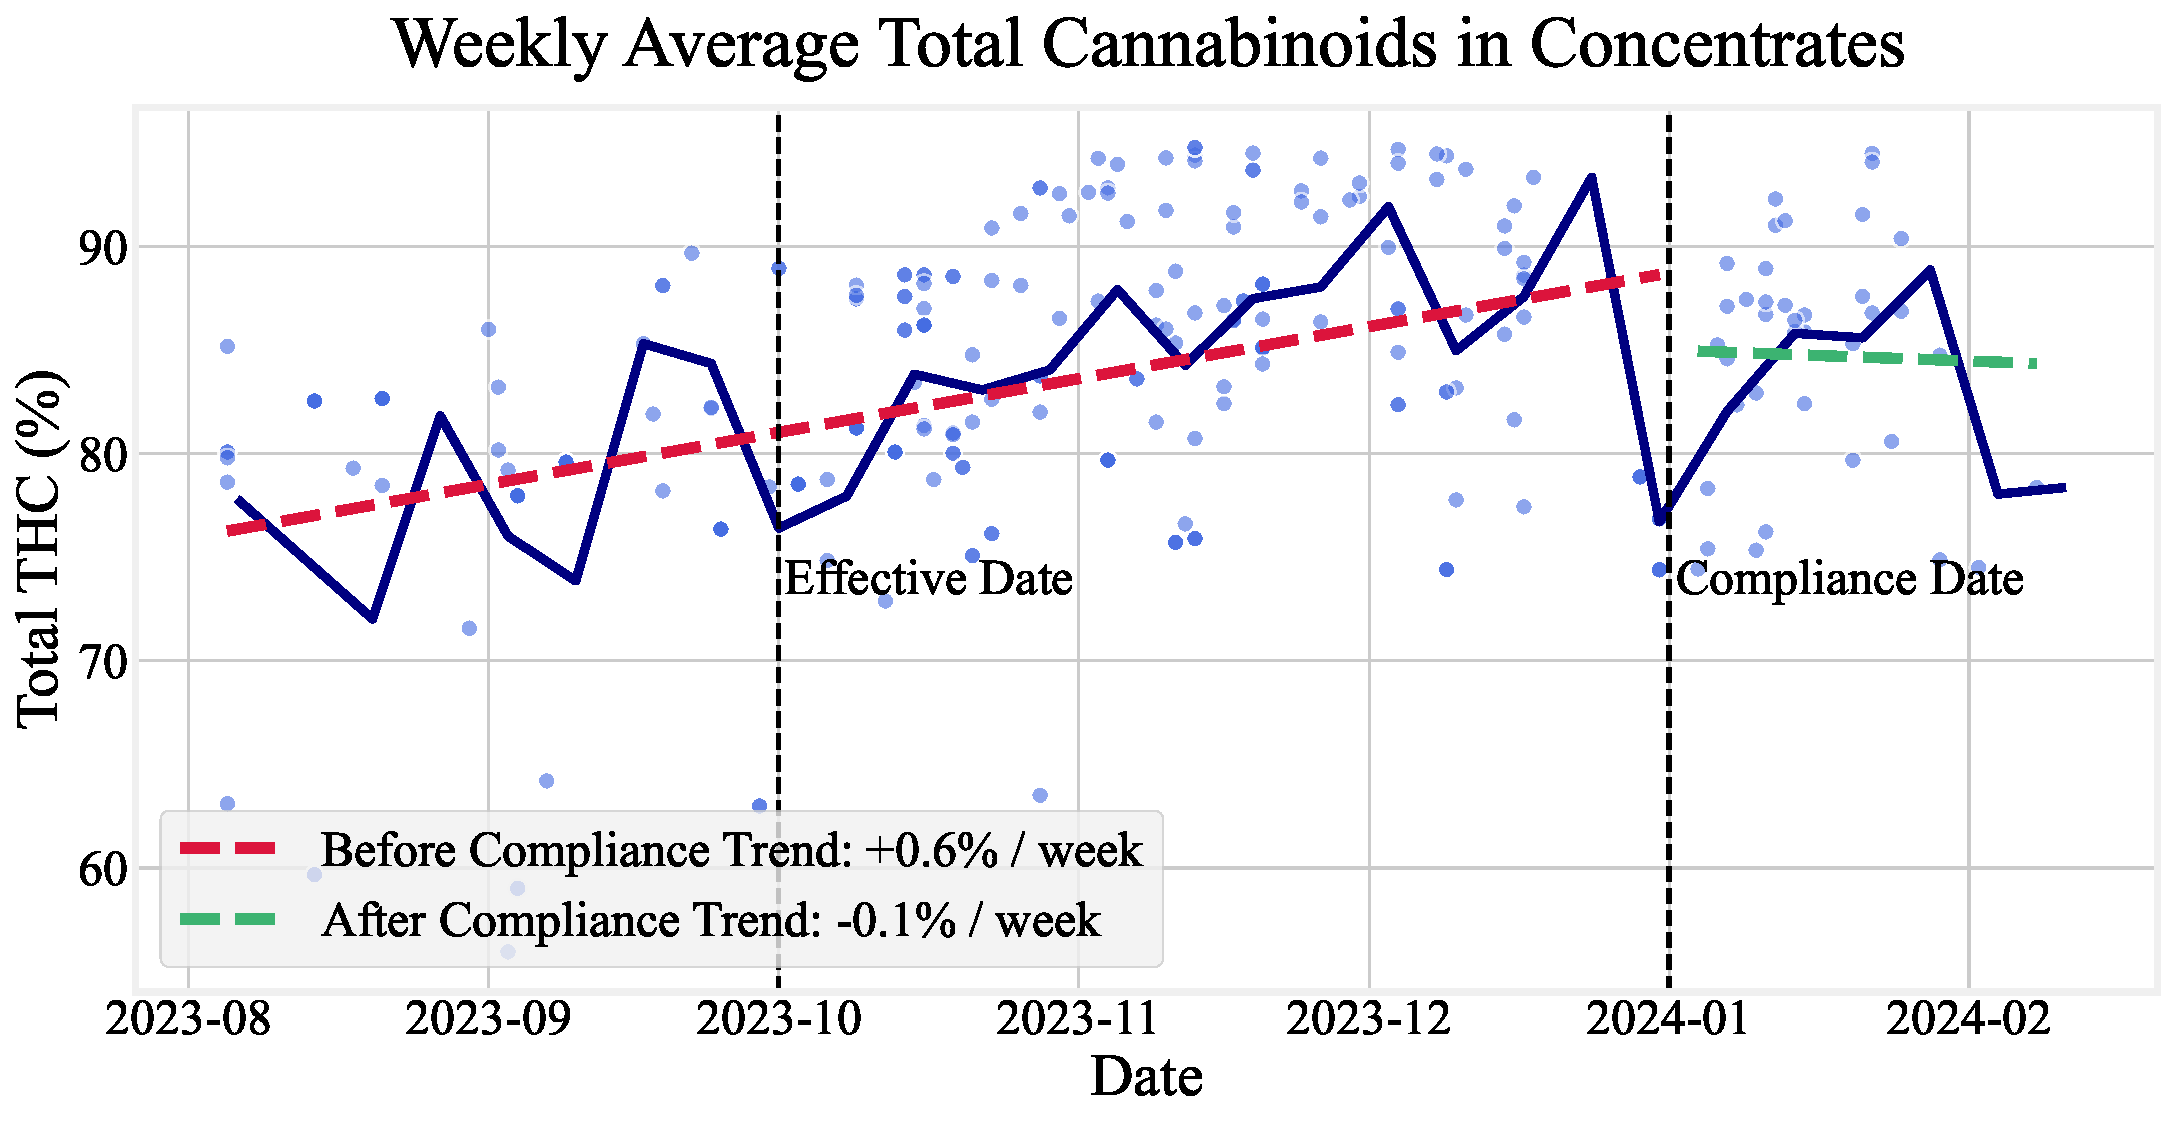
\includegraphics[width=\linewidth]{figures/total-cannabinoids-concentrates-timeseries.pdf}

% Total THC  in flower timeseries
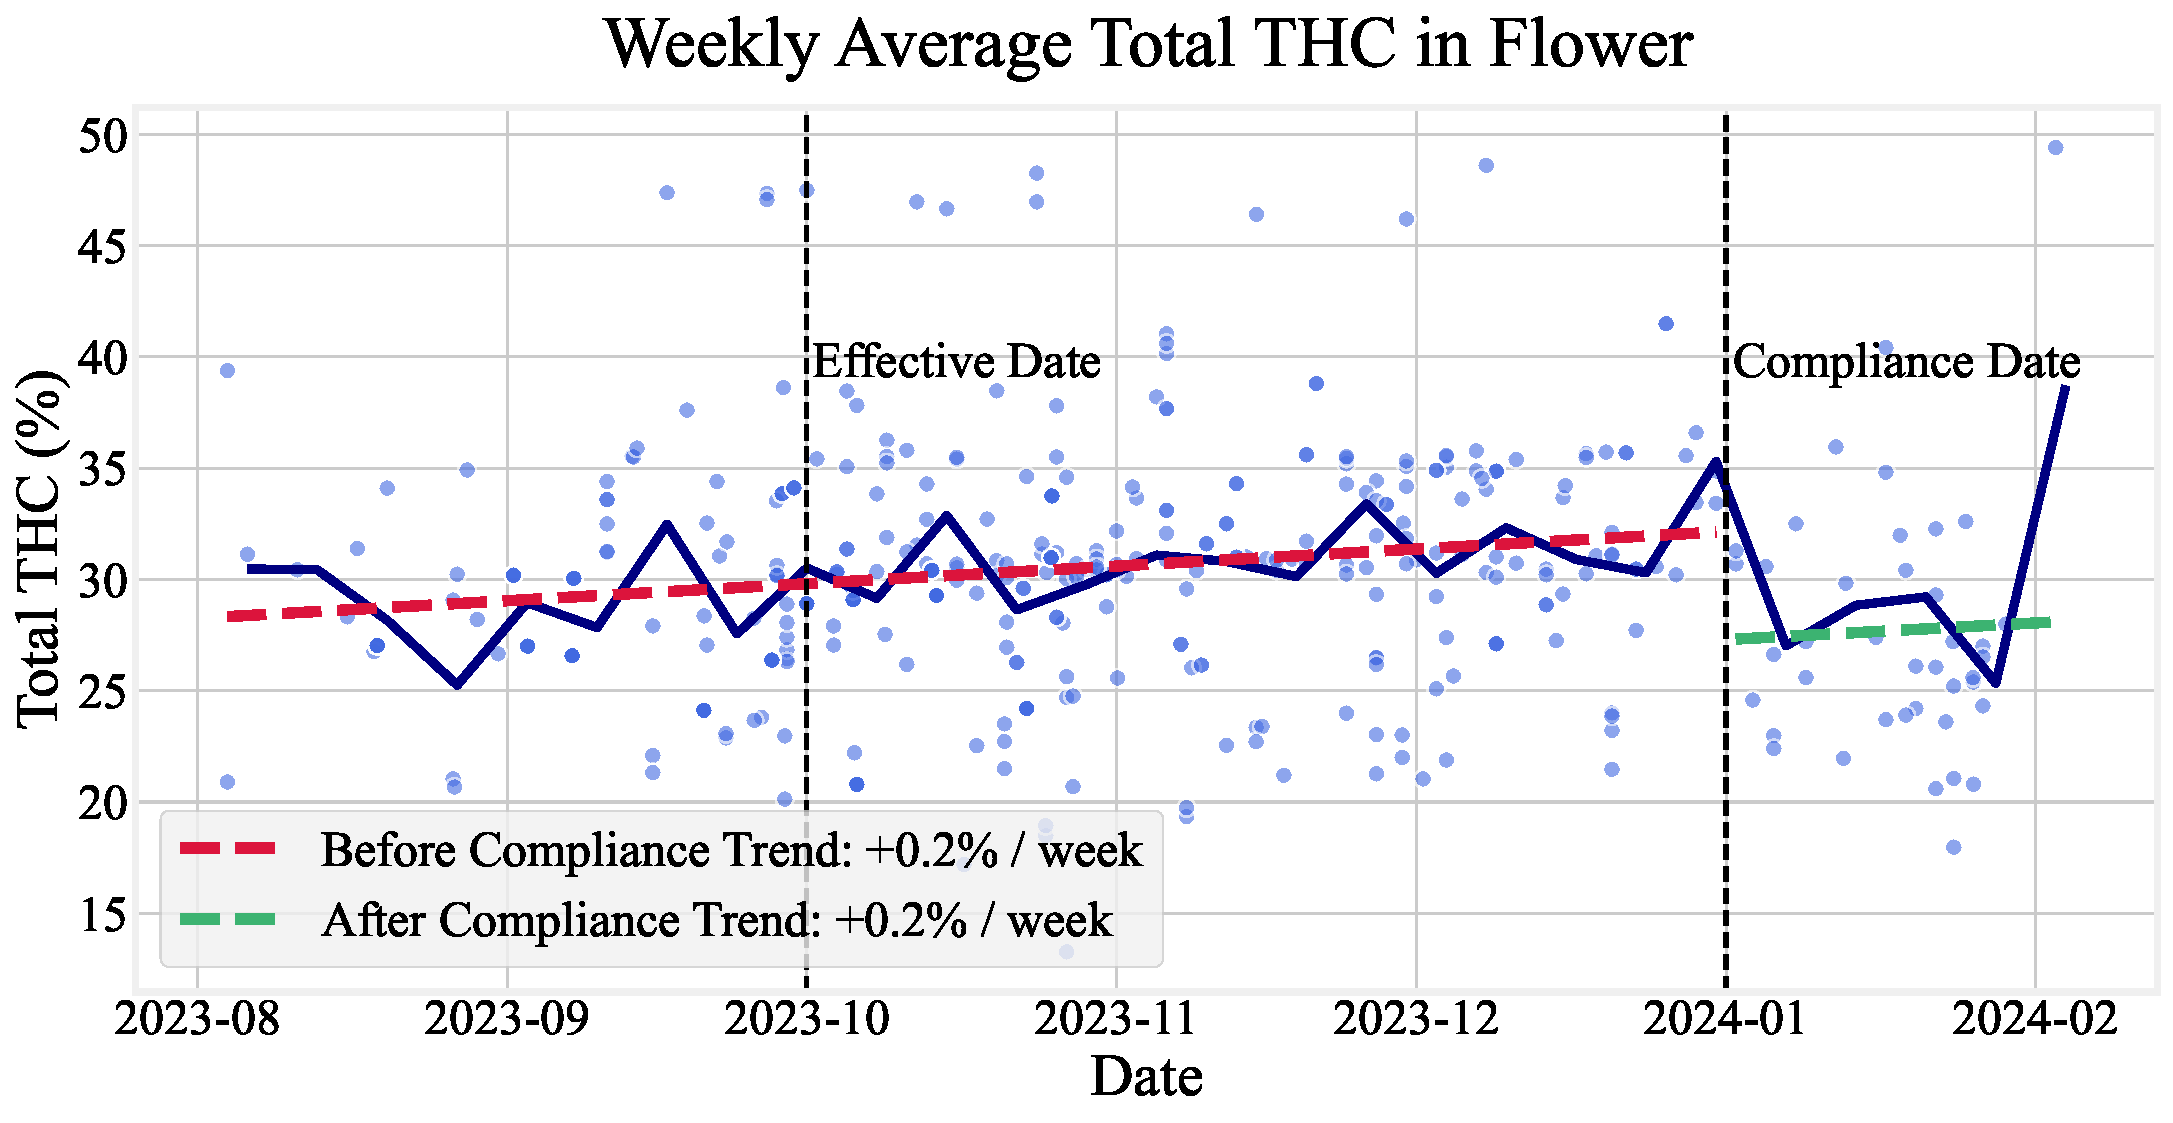
\includegraphics[width=\linewidth]{figures/total-thc-flower-timeseries.pdf}

\vspace{2\baselineskip}

% Total THC in concentrates timeseries
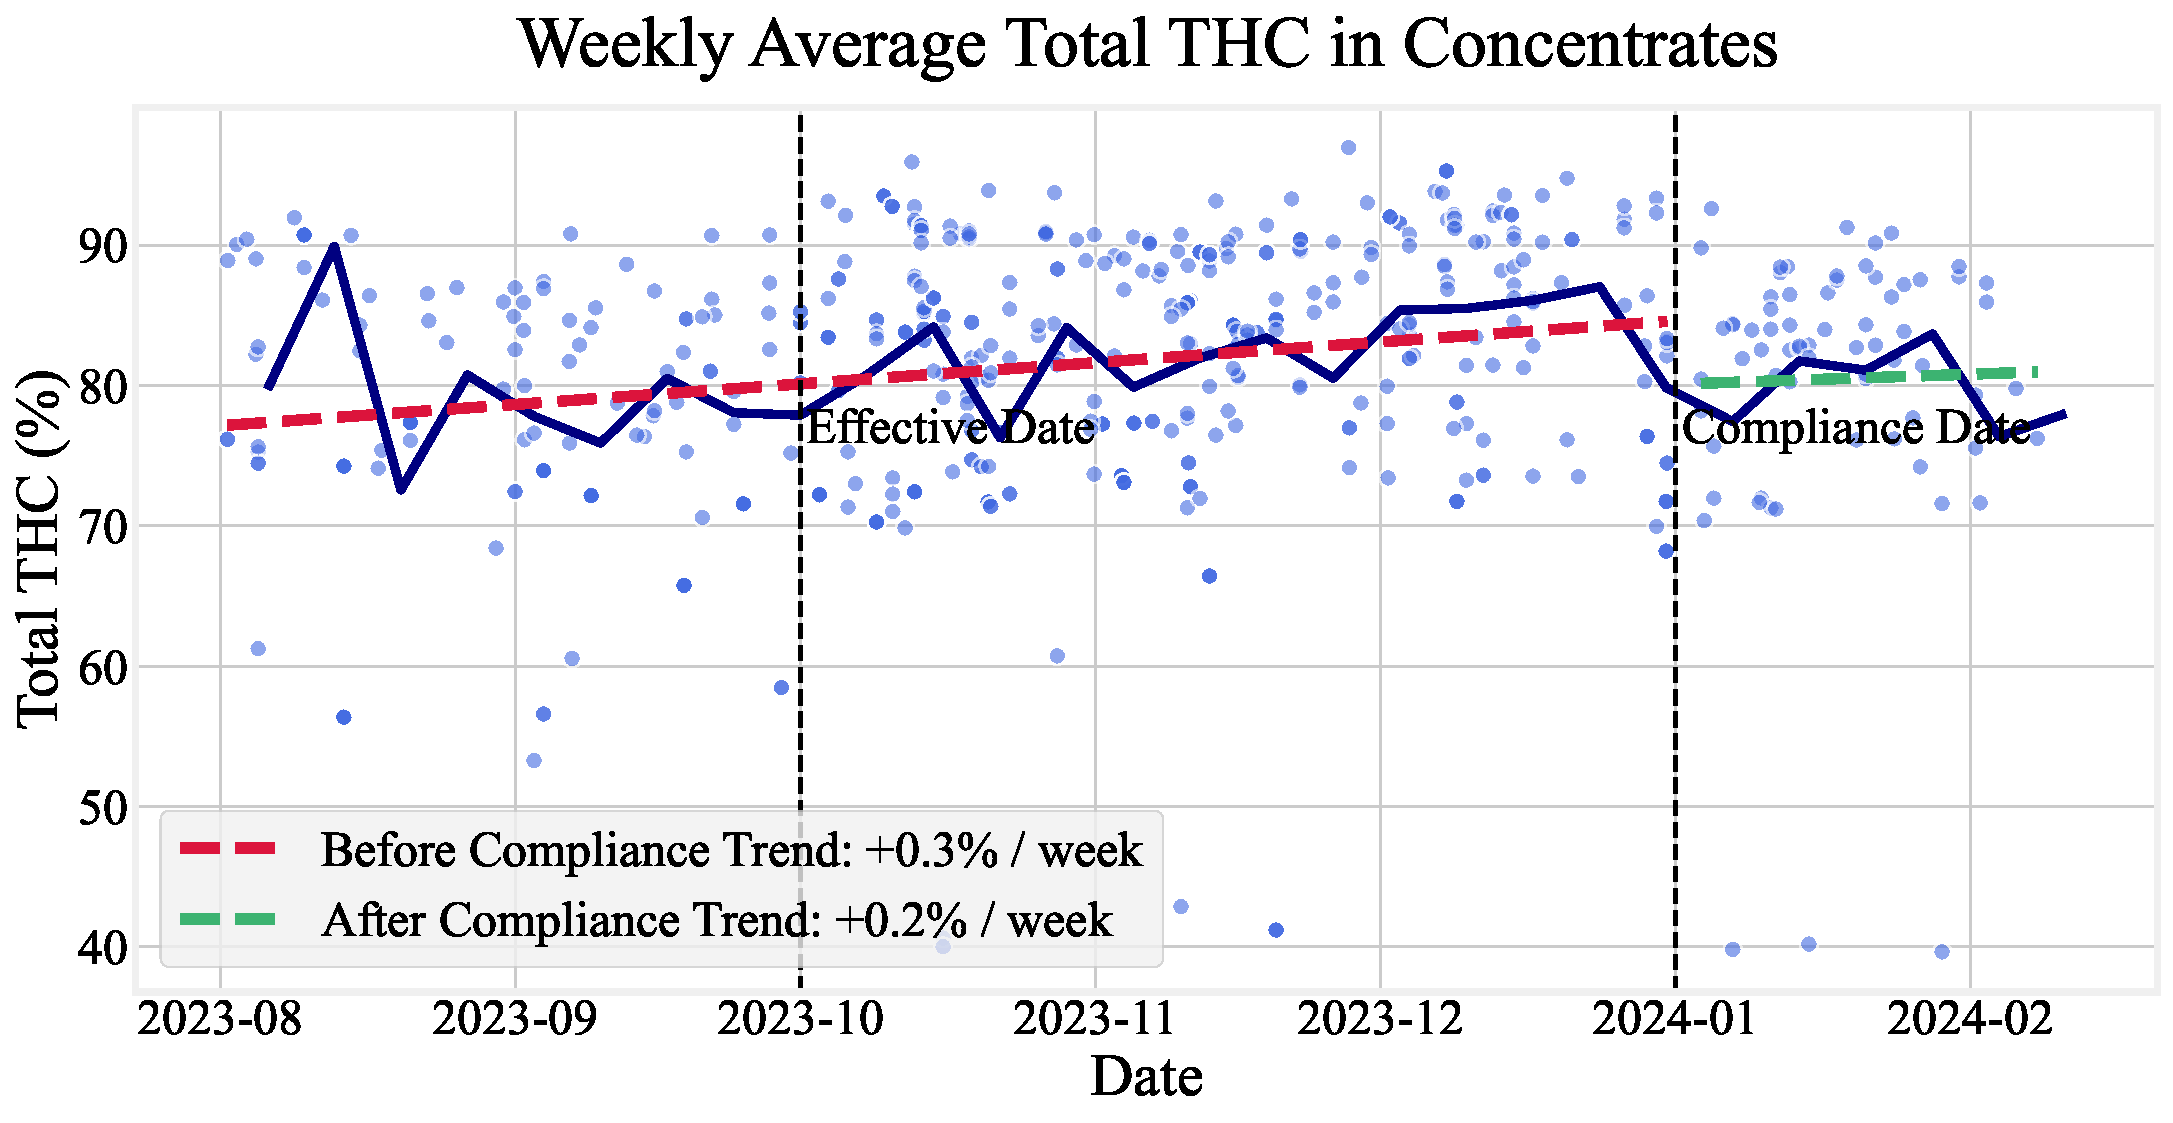
\includegraphics[width=\linewidth]{figures/total-thc-concentrates-timeseries.pdf}

\vspace{2\baselineskip}

% Total terpenes in flower timeseries
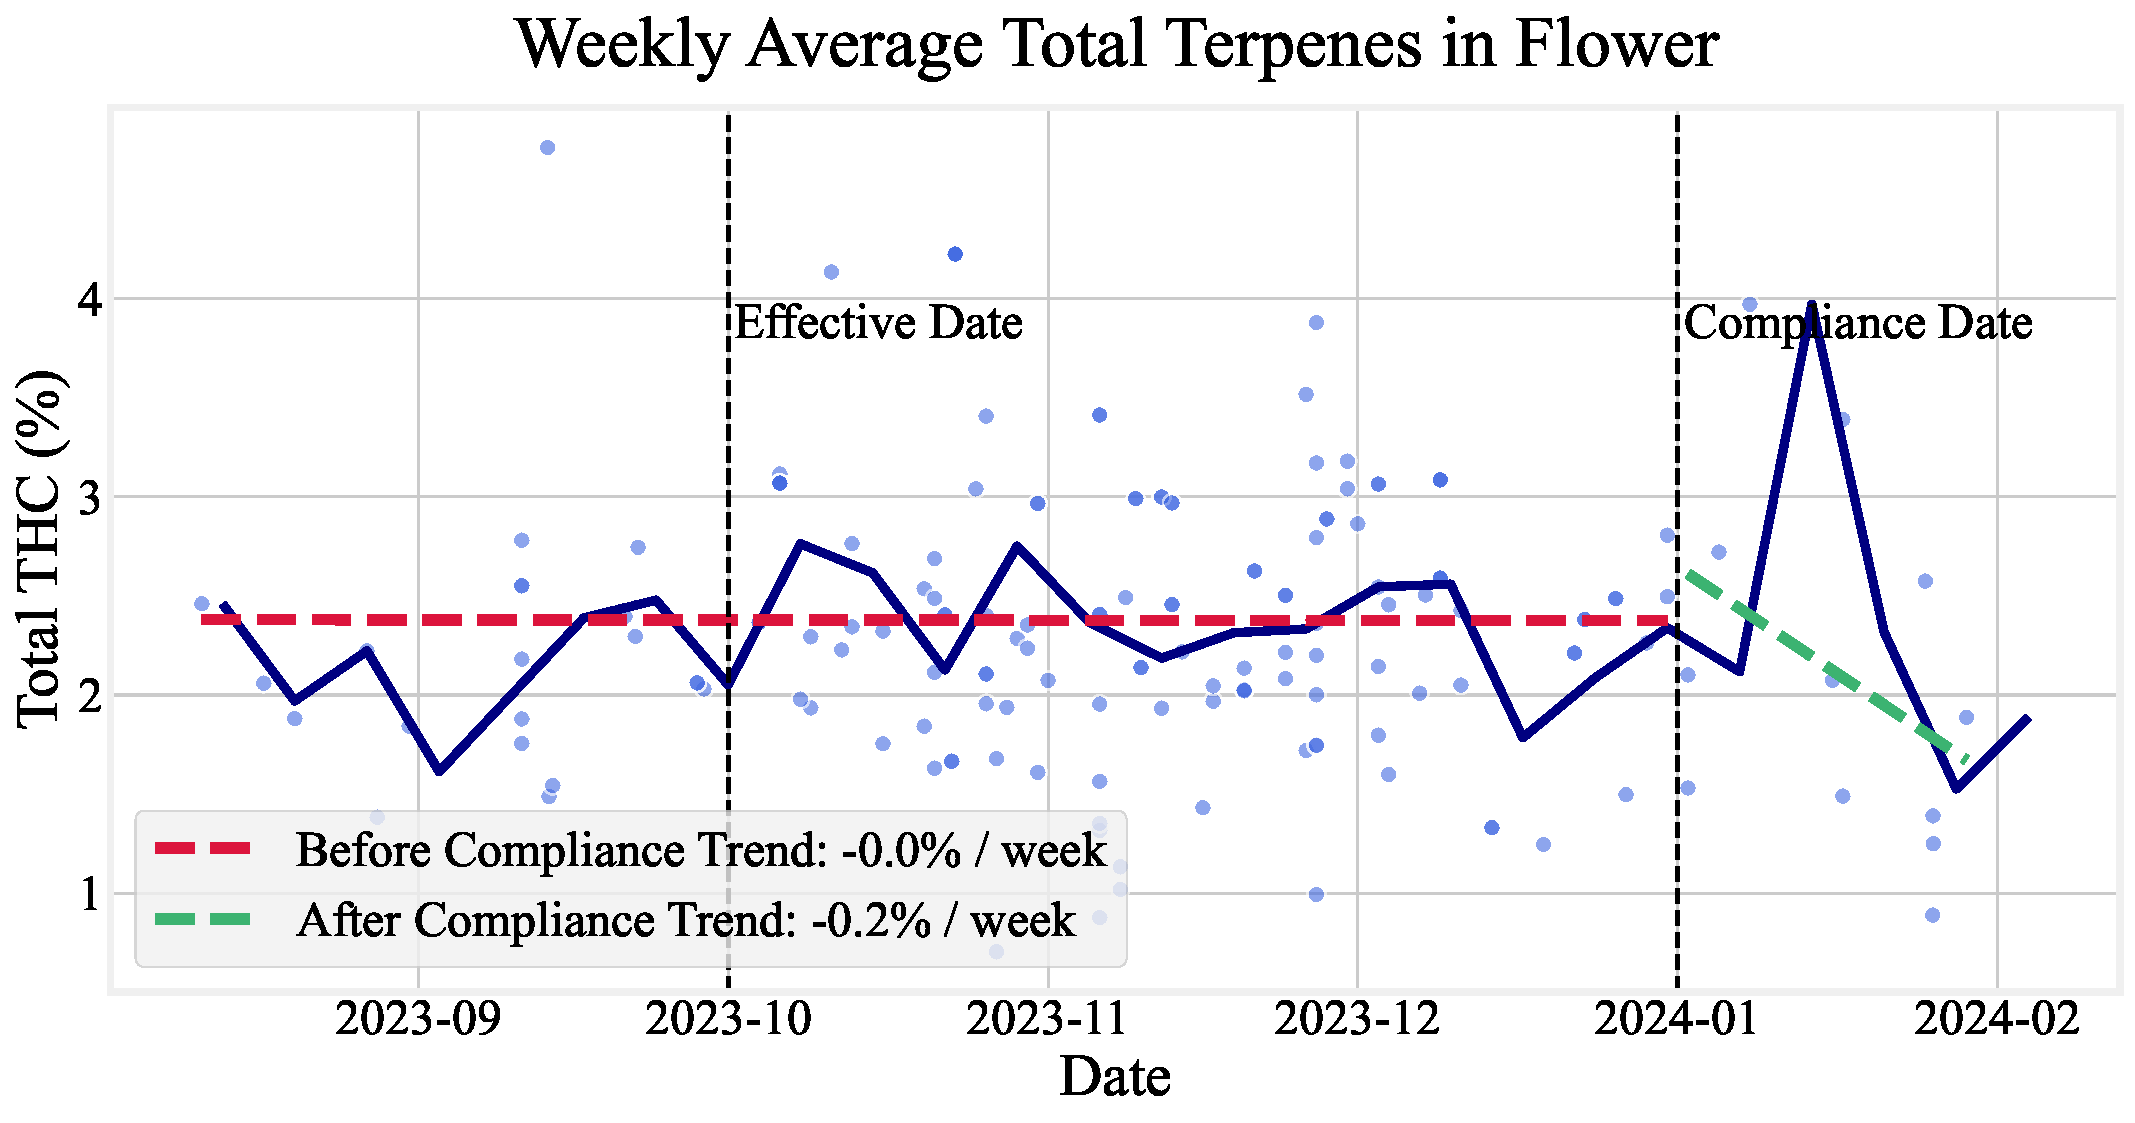
\includegraphics[width=\linewidth]{figures/total-terpenes-flower-timeseries.pdf}

\vspace{2\baselineskip}

% Total terpenes in concentrates timeseries
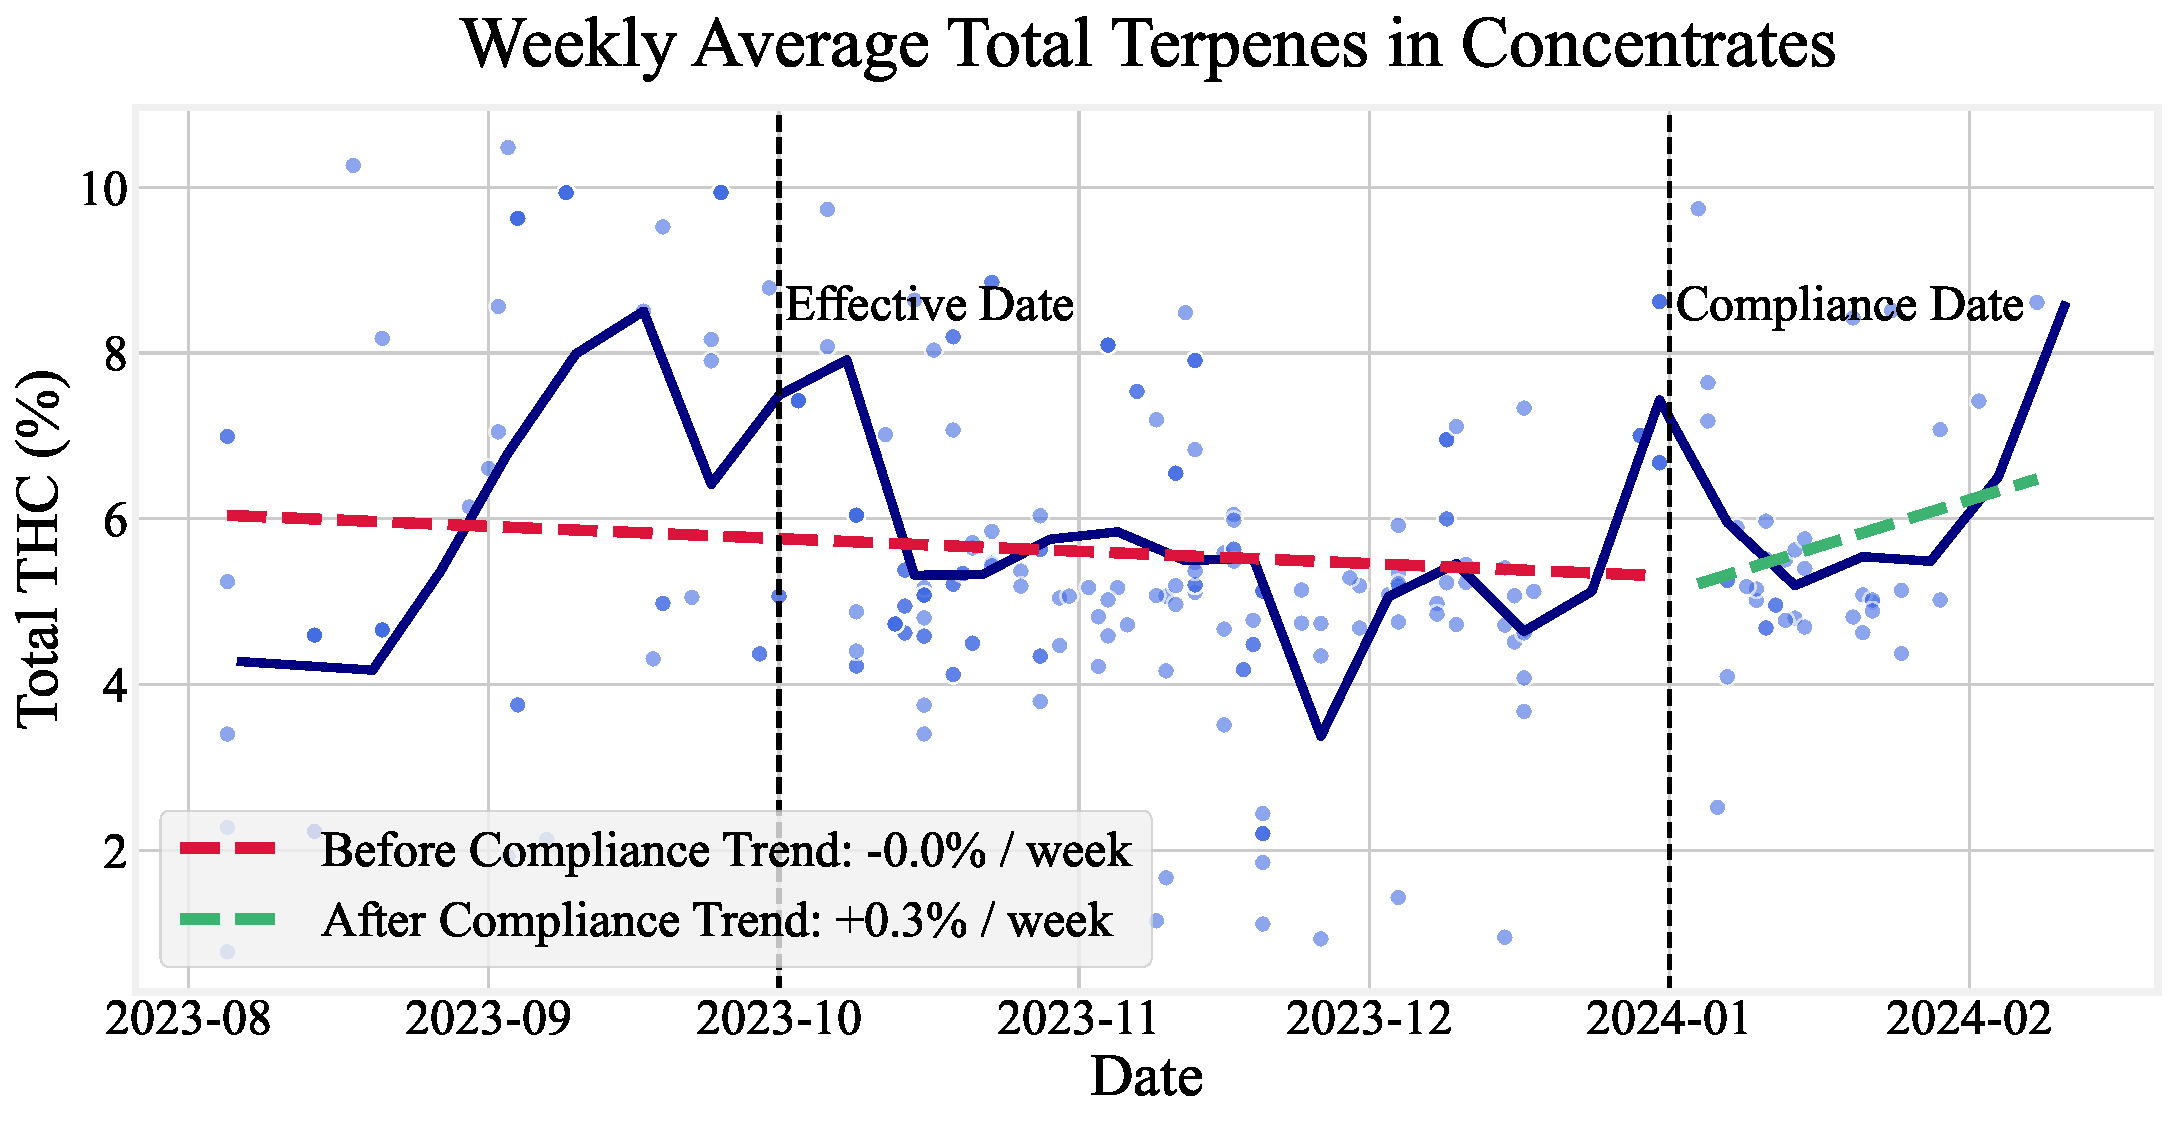
\includegraphics[width=\linewidth]{figures/total-terpenes-concentrates-timeseries.pdf}

\vspace{2\baselineskip}

% Total THC by lab timeseries.
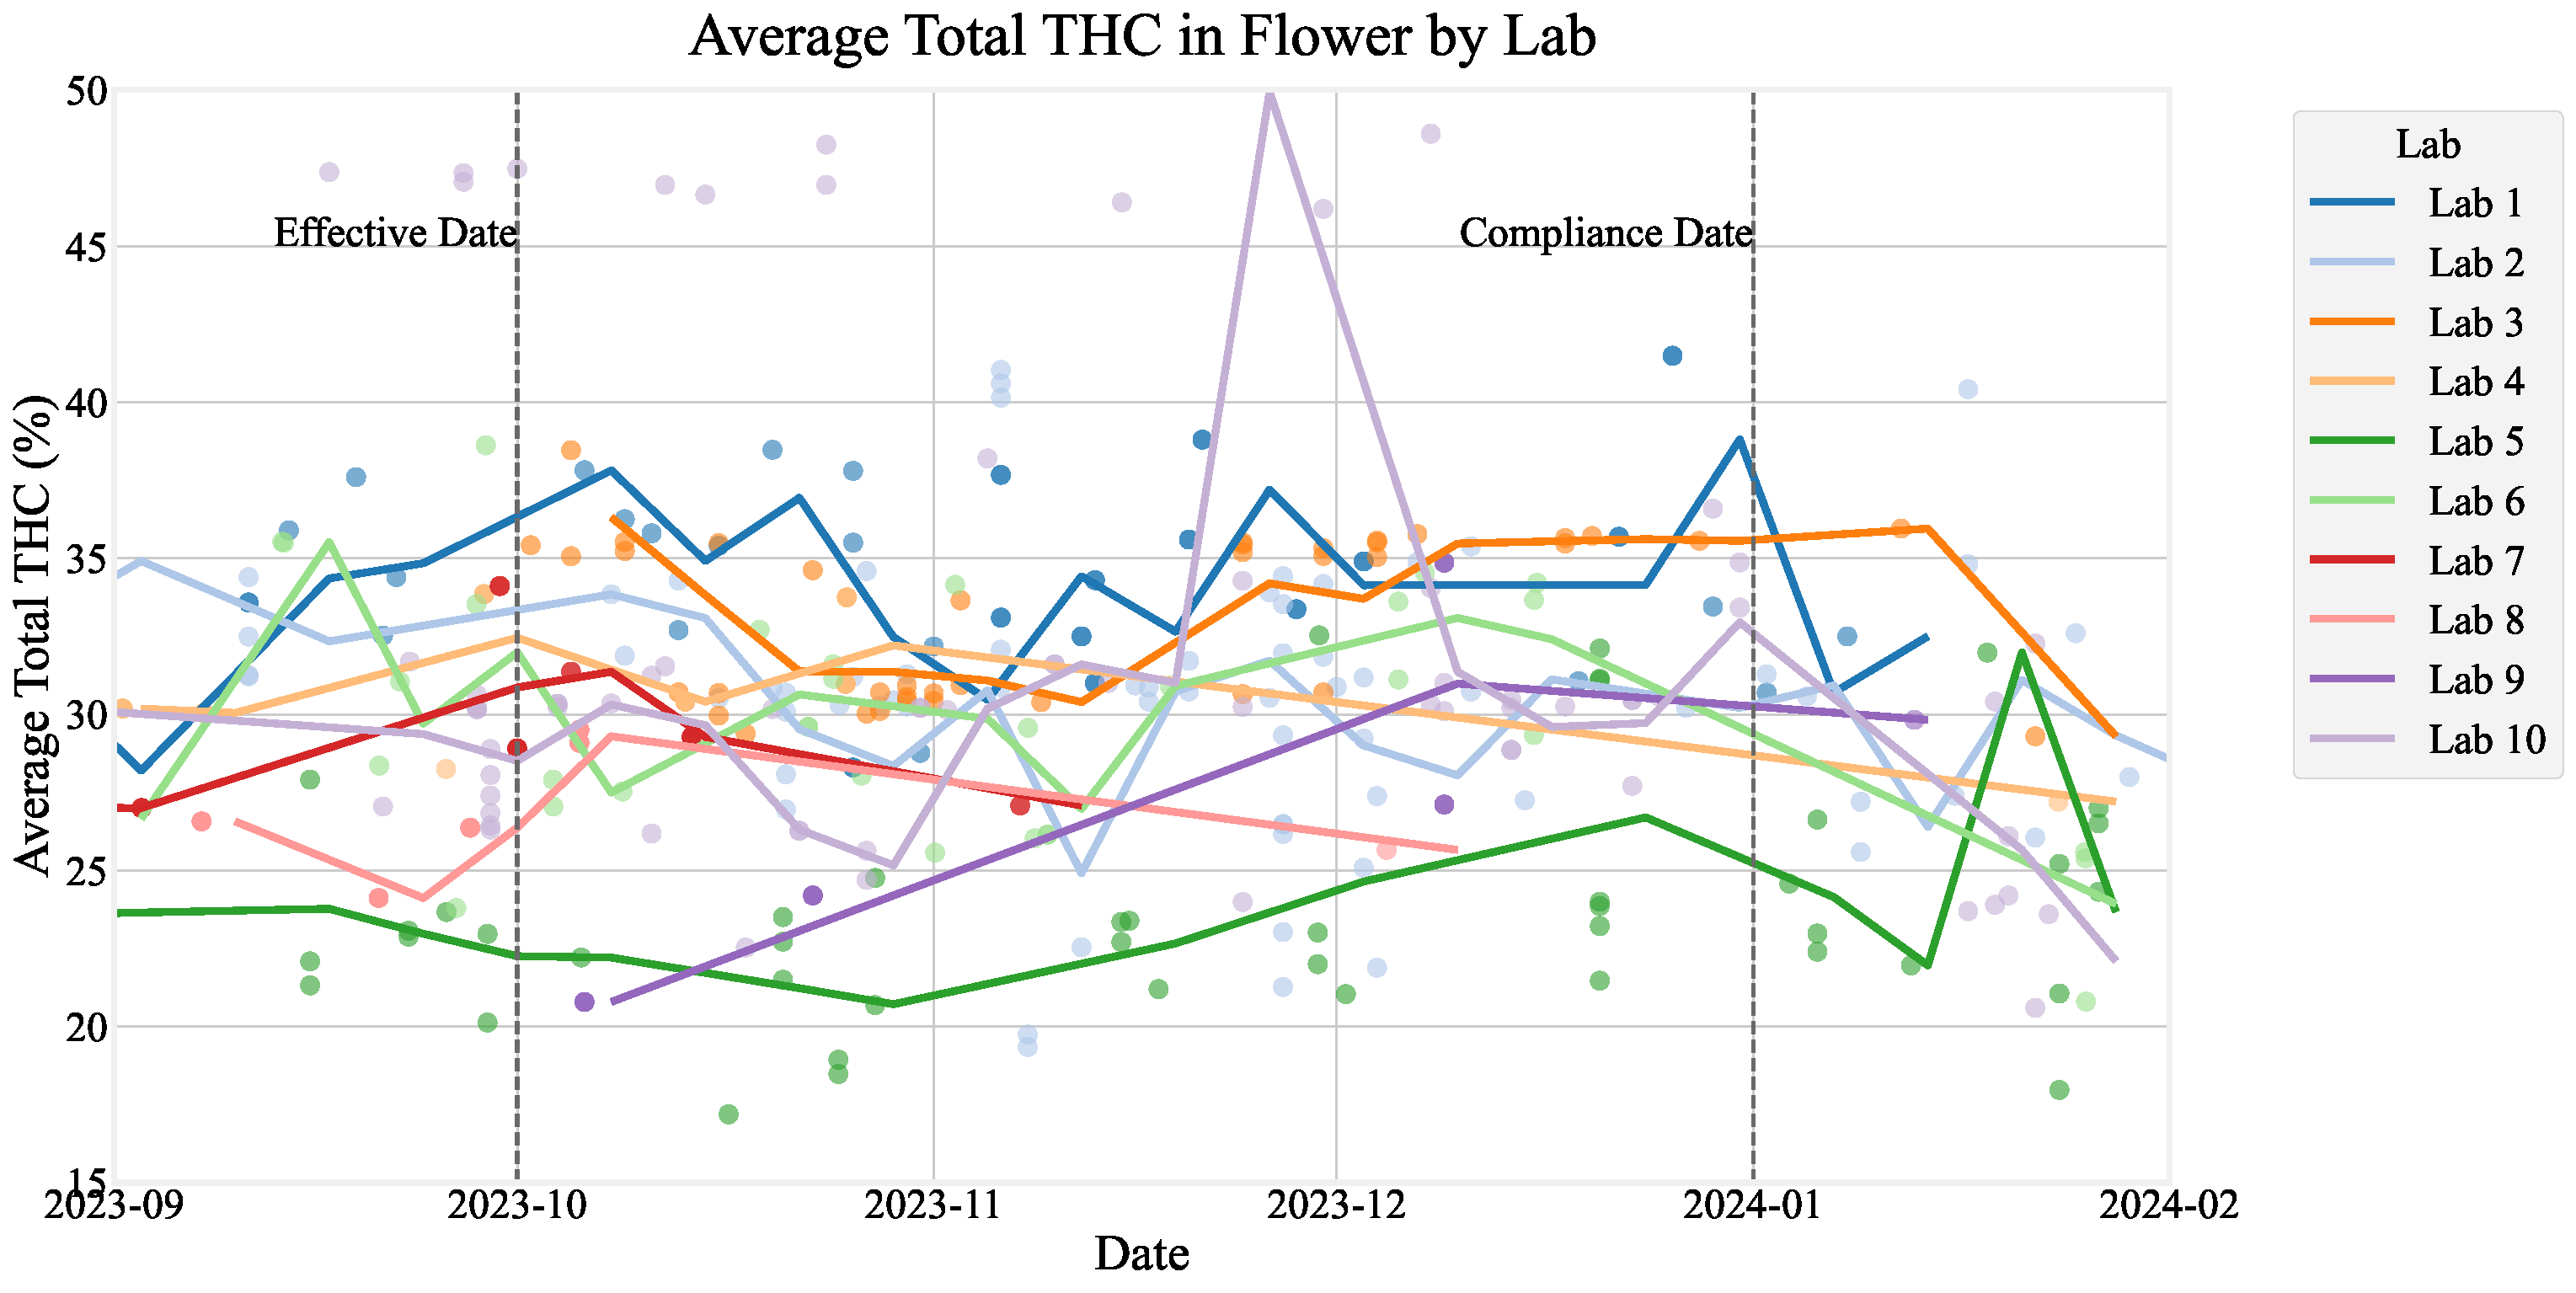
\includegraphics[width=\linewidth]{figures/total-thc-by-lab-timeseries.pdf}

\vspace{2\baselineskip}

% Total THC histogram.
\begin{center}
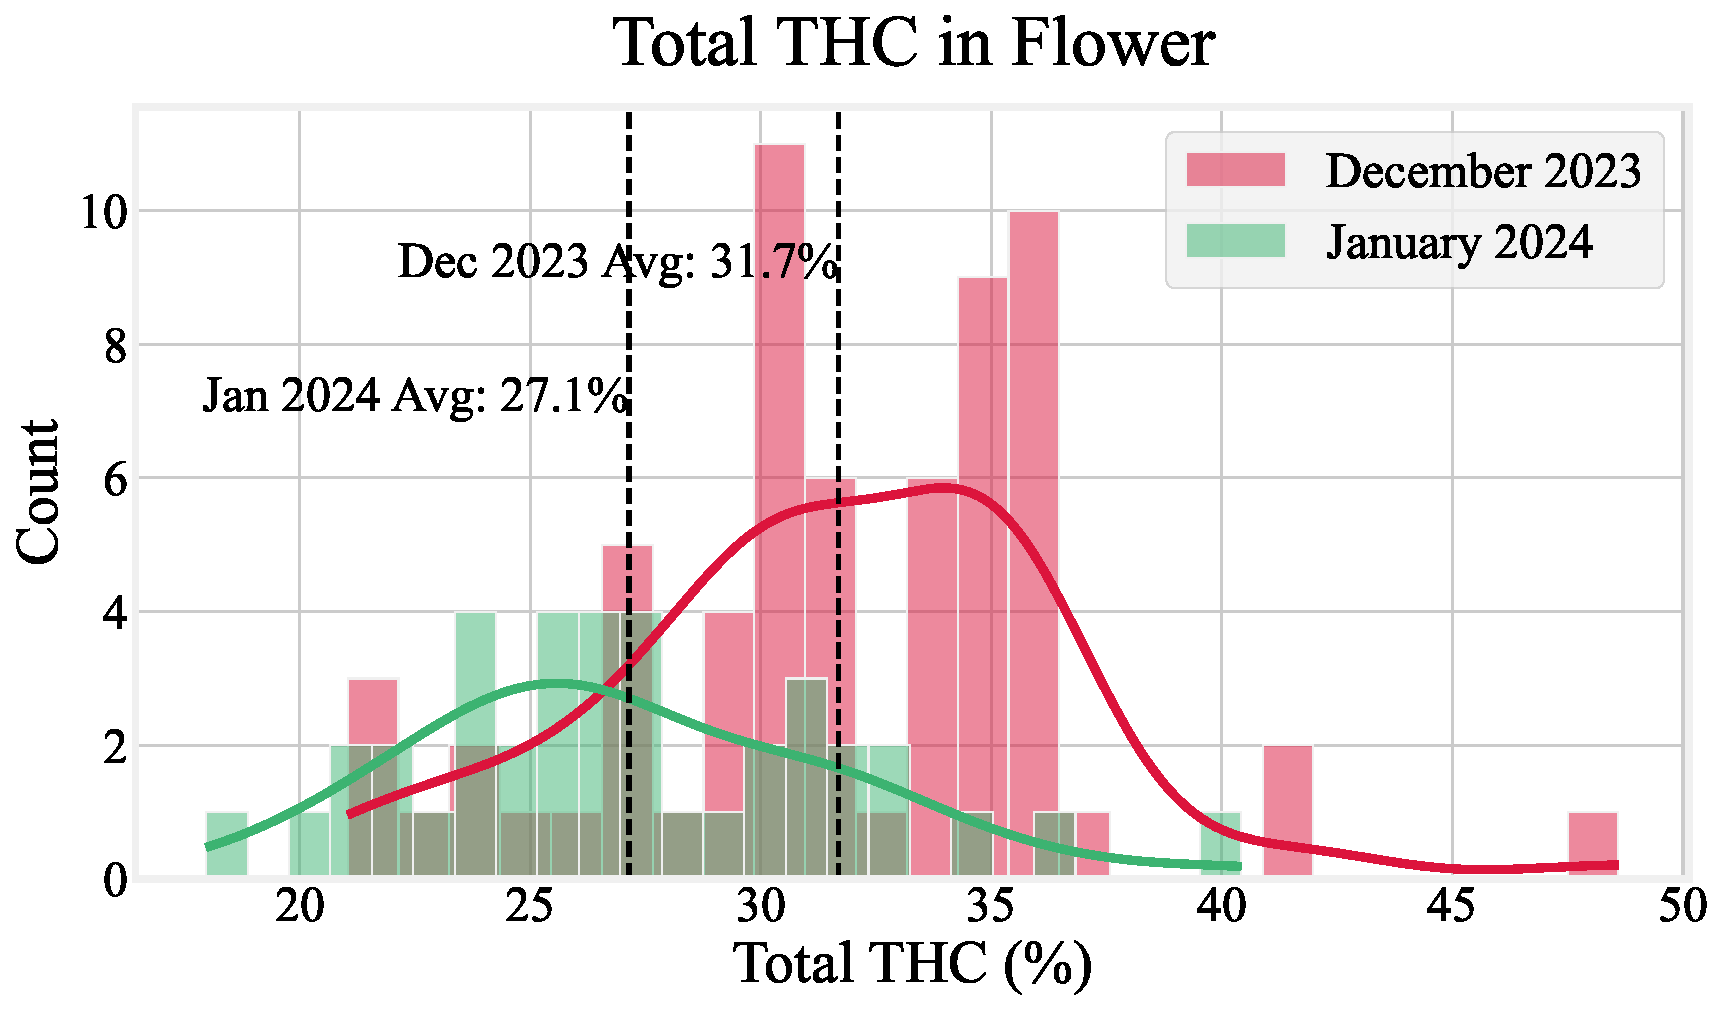
\includegraphics[width=0.8\linewidth]{figures/total-thc-histogram.pdf}
\end{center}


%---------------------------------%
% Average concentrations
%---------------------------------%

\newpage

Finally, we can examine the average concentration of cannabinoids by category in December 2023 compared to January 2024.

\noindent%
\begin{minipage}[t]{0.45\textwidth}

   % December 2023 Compounds Table
  {
    \tiny
    \vspace{1\baselineskip}
    \subfile{stats/compounds-2023-12}
  }

\end{minipage}\hspace{0.05\textwidth}
%
\begin{minipage}[t]{0.45\textwidth}

  % January 2024 Compounds Table
  {
    \tiny
    \vspace{1\baselineskip}
    \subfile{stats/compounds-2024-01}
  }

\end{minipage}


%---------------------------------%
% Lab Analysis
%---------------------------------%


%---------------------------------%
% Producer Analysis
%---------------------------------%


%---------------------------------%
% References
%---------------------------------%
%\newpage
%\nocite{*}
%\bibliography{references}

%---------------------------------%
% End of the Body
%---------------------------------%
\end{document}
